% Lines starting with a percent sign (%) are comments. LaTeX will 
% not process those lines. Similarly, everything after a percent 
% sign in a line is considered a comment. To produce a percent sign
% in the output, write \% (backslash followed by the percent sign). 
% ==================================================================
% Usage instructions:
% ------------------------------------------------------------------
% The file is heavily commented so that you know what the various
% commands do. Feel free to remove any comments you don't need from
% your own copy. When redistributing the example thesis file, please
% retain all the comments for the benefit of other thesis writers! 
% ==================================================================
% Compilation instructions: 
% ------------------------------------------------------------------
% Use pdflatex to compile! Input images are expected as PDF files.
% Example compilation:
% ------------------------------------------------------------------
% > pdflatex thesis-example.tex
% > bibtex thesis-example
% > pdflatex thesis-example.tex
% > pdflatex thesis-example.tex
% ------------------------------------------------------------------
% You need to run pdflatex multiple times so that all the cross-references
% are fixed. pdflatex will tell you if you need to re-run it (a warning
% will be issued)  
% ------------------------------------------------------------------
% Compilation has been tested to work in ukk.cs.hut.fi and kosh.hut.fi
% - if you have problems of missing .sty -files, then the local LaTeX
% environment does not have all the required packages installed.
% For example, when compiling in vipunen.hut.fi, you get an error that
% tikz.sty is missing - in this case you must either compile somewhere
% else, or you cannot use TikZ graphics in your thesis and must therefore
% remove or comment out the tikz package and all the tikz definitions. 
% ------------------------------------------------------------------

% Document class for the thesis is report
% ------------------------------------------------------------------
% You can change this but do so at your own risk - it may break other things.
% Note that the option pdftext is used for pdflatex; there is no
% pdflatex option. 
% ------------------------------------------------------------------
\documentclass[12pt,a4paper,oneside,pdftex]{report}

% The input files (tex files) are encoded with the latin-1 encoding 
% (ISO-8859-1 works). Change the latin1-option if you use UTF8 
% (at some point LaTeX did not work with UTF8, but I'm not sure
% what the current situation is) 
\usepackage[latin1]{inputenc}
% OT1 font encoding seems to work better than T1. Check the rendered
% PDF file to see if the fonts are encoded properly as vectors (instead
% of rendered bitmaps). You can do this by zooming very close to any letter 
% - if the letter is shown pixelated, you should change this setting 
% (try commenting out the entire line, for example).  
\usepackage[OT1]{fontenc}
% The babel package provides hyphenating instructions for LaTeX. Give
% the languages you wish to use in your thesis as options to the babel
% package (as shown below). You can remove any language you are not
% going to use.
% Examples of valid language codes: english (or USenglish), british, 
% finnish, swedish; and so on.
\usepackage[finnish,english]{babel}


% Optional packages
% ------------------------------------------------------------------
% Select those packages that you need for your thesis. You may delete
% or comment the rest.

% Natbib allows you to select the format of the bibliography references.
% The first example uses numbered citations: 
\usepackage[square,sort&compress,numbers]{natbib}
% The second example uses author-year citations.
% If you use author-year citations, change the bibliography style (below); 
% acm style does not work with author-year citations.
% Also, you should use~\citet (cite in text) when you wish to refer
% to the author directly (\citet{blaablaa} said blaa blaa), and 
%~\citep when you wish to refer similarly than with numbered citations
% (It has been said that blaa blaa~\citep{blaablaa}).
% \usepackage[square]{natbib}

% The alltt package provides an all-teletype environment that acts
% like verbatim but you can use LaTeX commands in it. Uncomment if 
% you want to use this environment. 
% \usepackage{alltt}

% The eurosym package provides a euro symbol. Use with \euro{}
\usepackage{eurosym} 

% Verbatim provides a standard teletype environment that renderes
% the text exactly as written in the tex file. Useful for code
% snippets (although you can also use the listings package to get
% automatic code formatting). 
\usepackage{verbatim}

% The listing package provides automatic code formatting utilities
% so that you can copy-paste code examples and have them rendered
% nicely. See the package documentation for details.
% \usepackage{listings}

% The fancuvrb package provides fancier verbatim environments 
% (you can, for example, put borders around the verbatim text area
% and so on). See package for details.
% \usepackage{fancyvrb}

% Supertabular provides a tabular environment that can span multiple 
% pages. 
%\usepackage{supertabular}
% Longtable provides a tabular environment that can span multiple 
% pages. This is used in the example acronyms file. 
\usepackage{longtable}

% The fancyhdr package allows you to set your the page headers 
% manually, and allows you to add separator lines and so on. 
% Check the package documentation. 
% \usepackage{fancyhdr}

% Subfigure package allows you to use subfigures (i.e. many subfigures
% within one figure environment). These can have different labels and
% they are numbered automatically. Check the package documentation. 
\usepackage{subfigure}

% The titlesec package can be used to alter the look of the titles 
% of sections, chapters, and so on. This example uses the ``medium'' 
% package option which sets the titles to a medium size, making them
% a bit smaller than what is the default. You can fine-tune the 
% title fonts and sizes by using the package options. See the package
% documentation.
\usepackage[medium]{titlesec}

% The TikZ package allows you to create professional technical figures.
% The learning curve is quite steep, but it is definitely worth it if 
% you wish to have really good-looking technical figures. 
\usepackage{tikz}
% You also need to specify which TikZ libraries you use
\usetikzlibrary{positioning}
\usetikzlibrary{calc}
\usetikzlibrary{arrows}
\usetikzlibrary{decorations.pathmorphing,decorations.markings}
\usetikzlibrary{shapes}
\usetikzlibrary{patterns}


% The aalto-thesis package provides typesetting instructions for the
% standard master's thesis parts (abstracts, front page, and so on)
% Load this package second-to-last, just before the hyperref package.
% Options that you can use: 
%   mydraft - renders the thesis in draft mode. 
%             Do not use for the final version. 
%   doublenumbering - [optional] number the first pages of the thesis
%                     with roman numerals (i, ii, iii, ...); and start
%                     arabic numbering (1, 2, 3, ...) only on the 
%                     first page of the first chapter
%   twoinstructors  - changes the title of instructors to plural form
%   twosupervisors  - changes the title of supervisors to plural form
% \usepackage[mydraft]{aalto-thesis}
\usepackage[mydraft,doublenumbering,twoinstructors]{aalto-thesis}
%\usepackage{aalto-thesis}


% Hyperref
% ------------------------------------------------------------------
% Hyperref creates links from URLs, for references, and creates a
% TOC in the PDF file.
% This package must be the last one you include, because it has
% compatibility issues with many other packages and it fixes
% those issues when it is loaded.   
\RequirePackage[pdftex]{hyperref}
% Setup hyperref so that links are clickable but do not look 
% different
\hypersetup{colorlinks=false,raiselinks=false,breaklinks=true}
\hypersetup{pdfborder={0 0 0}}
\hypersetup{bookmarksnumbered=true}
% The following line suggests the PDF reader that it should show the 
% first level of bookmarks opened in the hierarchical bookmark view. 
\hypersetup{bookmarksopen=true,bookmarksopenlevel=1}
% Hyperref can also set up the PDF metadata fields. These are
% set a bit later on, after the thesis setup.   


% Thesis setup
% ==================================================================
% Change these to fit your own thesis.
% \COMMAND always refers to the English version;
% \FCOMMAND refers to the Finnish version; and
% \SCOMMAND refers to the Swedish version.
% You may comment/remove those language variants that you do not use
% (but then you must not include the abstracts for that language)
% ------------------------------------------------------------------
% If you do not find the command for a text that is shown in the cover page or
% in the abstract texts, check the aalto-thesis.sty file and locate the text
% from there. 
% All the texts are configured in language-specific blocks (lots of commands
% that look like this: \renewcommand{\ATCITY}{Espoo}.
% You can just fix the texts there. Just remember to check all the language
% variants you use (they are all there in the same place). 
% ------------------------------------------------------------------
\newcommand{\TITLE}{Privacy Implications of Wireless\\ Network Probing}
\newcommand{\FTITLE}{Yksityisyydensuoja langattomissa verkoissa}
\newcommand{\SUBTITLE}{}
\newcommand{\FSUBTITLE}{}
\newcommand{\DATE}{August 5, 2014}
\newcommand{\FDATE}{5. elokuuta 2014}

% Supervisors and instructors
% ------------------------------------------------------------------
% If you have two supervisors, write both names here, separate them with a 
% double-backslash
% Also remember to add the package option ``twosupervisors'' or
% ``twoinstructors'' to the aalto-thesis package so that the titles are in
% plural.

\newcommand{\SUPERVISOR}{Professor Tuomas Aura}
\newcommand{\FSUPERVISOR}{Professori Tuomas Aura}

\newcommand{\INSTRUCTOR}{Professor Christopher Kruegel\\Professor Giovanni Vigna}
\newcommand{\FINSTRUCTOR}{Professori Christopher Kruegel\\Professori Giovanni Vigna}

\newcommand{\COVERSUPERVISOR}{Professor Tuomas Aura, Aalto University}
\newcommand{\COVERINSTRUCTOR}{Professor Christopher Kruegel, UC Santa Barbara\\Professor Giovanni Vigna, UC Santa Barbara}


% Other stuff
% ------------------------------------------------------------------
\newcommand{\PROFESSORSHIP}{Data Communication Software}
\newcommand{\FPROFESSORSHIP}{Tietoliikenneohjelmistot}

% Professorship code is the same in all languages
\newcommand{\PROFCODE}{T-110}
\newcommand{\KEYWORDS}{}
\newcommand{\FKEYWORDS}{}

\newcommand{\LANGUAGE}{English}
\newcommand{\FLANGUAGE}{Englanti}

% Author is the same for all languages
\newcommand{\AUTHOR}{Pekko Lipsanen}


% Currently the English versions are used for the PDF file metadata
% Set the PDF title
\hypersetup{pdftitle={\TITLE\ \SUBTITLE}}
% Set the PDF author
\hypersetup{pdfauthor={\AUTHOR}}
% Set the PDF keywords
\hypersetup{pdfkeywords={\KEYWORDS}}
% Set the PDF subject
\hypersetup{pdfsubject={Master's Thesis}}


% Layout settings
% ------------------------------------------------------------------

% Use this to control how much space there is between each line of text.
% 1 is normal (no extra space), 1.3 is about one-half more space, and
% 1.6 is about double line spacing.  
% \linespread{1} % This is the default
% \linespread{1.3}

% Bibliography style
% acm style gives you a basic reference style. It works only with numbered
% references.
% \bibliographystyle{acm}
% Plainnat is a plain style that works with both numbered and name citations.
\bibliographystyle{plainnat}


% Extra hyphenation settings
% ------------------------------------------------------------------
% You can list here all the files that are not hyphenated correctly.
% You can provide many \hyphenation commands and/or separate each word
% with a space inside a single command. Put hyphens in the places where
% a word can be hyphenated.
% Note that (by default) LaTeX will not hyphenate words that already
% have a hyphen in them (for example, if you write ``structure-modification 
% operation'', the word structure-modification will never be hyphenated).
% You need a special package to hyphenate those words.
% \hyphenation{di-gi-taa-li-sta yksi-suun-tai-sta}


% The preamble ends here, and the document begins. 
% Place all formatting commands and such before this line.
% ------------------------------------------------------------------
\begin{document}
% This command adds a PDF bookmark to the cover page. You may leave
% it out if you don't like it...
\pdfbookmark[0]{Cover page}{bookmark.0.cover}
% This command is defined in aalto-thesis.sty. It controls the page 
% numbering based on whether the doublenumbering option is specified
\startcoverpage

% Cover page
% ------------------------------------------------------------------
% Options: finnish, english, and swedish
% These control in which language the cover-page information is shown
\coverpage{english}


% Abstracts
% ------------------------------------------------------------------
% Include an abstract in the language that the thesis is written in,
% and if your native language is Finnish or Swedish, one in that language.

% Abstract in English
% ------------------------------------------------------------------
\thesisabstract{english}{

}

% Abstract in Finnish
% ------------------------------------------------------------------
\thesisabstract{finnish}{

}

% Acknowledgements
% ------------------------------------------------------------------
% Select the language you use in your acknowledgements
\selectlanguage{english}

% Uncomment this line if you wish acknoledgements to appear in the 
% table of contents
%\addcontentsline{toc}{chapter}{Acknowledgements}

% The star means that the chapter isn't numbered and does not 
% show up in the TOC
\chapter*{Acknowledgements}

aalto, eurecom s3/nops, ucsb, speksi, WiGLE, everyone

\vskip 10mm

\noindent Espoo, \DATE
\vskip 5mm
\noindent\AUTHOR

% Acronyms
% ------------------------------------------------------------------
% Use \cleardoublepage so that IF two-sided printing is used 
% (which is not often for masters theses), then the pages will still
% start correctly on the right-hand side.
\cleardoublepage
% Example acronyms are placed in a separate file, acronyms.tex
\addcontentsline{toc}{chapter}{Abbreviations and Acronyms}
\chapter*{Abbreviations and Acronyms}

% The longtable environment should break the table properly to multiple pages, 
% if needed

\noindent
\begin{longtable}{@{}p{0.25\textwidth}p{0.7\textwidth}@{}}
BSSID & Basic Service Set Identifier \\
CCTV & Closed Circuit Television \\
EU & European Union \\
ESS & Extended Service Set \\
ESSID & Extended Service Set Identifier \\
HT & High throughput \\
IEEE & Institute of Electrical and Electronics Engineers \\
JSON & JavaScript Object Notation \\
MAC & Media Access Control \\
MCL & Markov Cluster \\
MITM & Man in the middle \\
QoS & Quality of Service \\
SSID & Service Set Identifier \\
SSL & Secure Sockets Layer \\
TLS & Transport Layer Security \\
UUID & Universally Unique Identifier \\
WLAN & Wireless Local Area Network \\
WPA & Wi-Fi Protected Access \\
WPS & Wi-Fi Protected Setup \\
\end{longtable}


% Table of contents
% ------------------------------------------------------------------
\cleardoublepage
% This command adds a PDF bookmark that links to the contents.
% You can use \addcontentsline{} as well, but that also adds contents
% entry to the table of contents, which is kind of redundant.
% The text ``Contents'' is shown in the PDF bookmark. 
\pdfbookmark[0]{Contents}{bookmark.0.contents}
\tableofcontents

% List of tables
% ------------------------------------------------------------------
% You only need a list of tables for your thesis if you have very 
% many tables. If you do, uncomment the following two lines.
% \cleardoublepage
% \listoftables

% Table of figures
% ------------------------------------------------------------------
% You only need a list of figures for your thesis if you have very 
% many figures. If you do, uncomment the following two lines.
% \cleardoublepage
% \listoffigures

% The following label is used for counting the prelude pages
\label{pages-prelude}
\cleardoublepage

%%%%%%%%%%%%%%%%% The main content starts here %%%%%%%%%%%%%%%%%%%%%
% ------------------------------------------------------------------
% This command is defined in aalto-thesis.sty. It controls the page 
% numbering based on whether the doublenumbering option is specified
\startfirstchapter

% Add headings to pages (the chapter title is shown)
\pagestyle{headings}


%%%%%%%%%%%%%%%%%%%%%%%%%%%%%%%%%%%%%%%%%%%%%%%%%%%%%%%%%%%%%%%%%%%%%%%%%%%%%%%


\chapter{Introduction}
\label{chapter:intro}

Wireless technology has been established well in everyday life. Most of the people have nowadays their own wireless network at home, and they use another one at school or at work. When traveling, hotels and airports almost always offer Wi-Fis, in many cases for free of charge. Wireless networks can also be found in shopping malls, restaurants, and even in airplanes, buses, and trains -- and the number of networks is only growing.

From the very nature of wireless networks, transferred data is always visible on the physical layer to everyone who is inside the range of the network. Compared to traditional on-wire networking, this creates worries for information security -- eavesdropping the cable is much harder. Lots of work has been done in order to make sure that actual transferred information, for example the content of web pages browsed, remains confident and is not visible for eavesdroppers. Such work includes, for example, standards for wireless network encryption.

However, we are interested in data exchange that happens before a device joins a wireless network. The device has not established any connections yet, so all the information is sent in plaintext, unencrypted, in public. This information includes at least the identifier of the device that is trying to connect to a network, and the network name it is trying to connect. Or, alternatively, the device can ask for information about all the networks in the range.

Manufacturers want to provide best possible user experience to their customers. A part of the experience is the ability to find a wireless network in the device's range, and to join fast to the network. Because of this, many devices scan continuously the airspace and try to find out if there are networks to join. An understandable goal means that devices might leak out data about users: the names of networks the device, or the user, would like to join.


\section{Scope}
\label{sec:scope}

In this thesis, we try to examine what information can be extracted from the pre-connection part of data transmission, and how the information can be used. Particular use cases include gathering information from passive monitoring and combining it with other dataset, for which we conduct a practical experiment. Together with that, we look for theoretical possibilities for active attacks exploiting mobile device's features.

The thesis is multidisciplinary: in addition to technical study, we will also examine the legal position of doing above-mentioned acts, and we are not limited to the technical side of the issue. In addition, we will look for technical countermeasures for found privacy and security threats: how the techniques we found can be circumvented, if someone wants to.

In the thesis, we do not take into account any other parts of data transmission. Especially outside the scope is traffic after connecting to network, such as user visiting web pages or reading his email.

For legal side, we do not try to give a worldwide detailed view. Instead, we focus on two major players, the United States and the European Union.

\section{Organization of thesis}

The thesis is organized as follows. In Chapter~\ref{chapter:protocol}, we tell how the 802.11 protocol, also known as Wi-Fi, works. We will see some important parts of the protocol in detail. In Chapter~\ref{chapter:profiling} we will examine how and why parts of wireless network protocols can be used for tracking and profiling users. Further, in Chapter~\ref{chapter:attacks} we will see how these features can be used in conducting active attacks and not only passive monitoring of devices.  In Chapter~\ref{chapter:legal} we study the legal status of discussed methods. Practical experiment of above-mentioned techniques is conducted in Chapter~\ref{chapter:practical}, and in Chapter~\ref{chapter:countermeasures} we will see how privacy-concerned users could be protected from the actions we have studied. Finally, in Chapter~\ref{chapter:conclusion} we conclude the thesis.


%%%%%%%%%%%%%%%%%%%%%%%%%%%%%%%%%%%%%%%%%%%%%%%%%%%%%%%%%%%%%%%%%%%%%%%%%%%%%%%


\chapter{The 802.11 wireless network protocol}
\label{chapter:protocol}

We will examine the protocols and data transmissions used inside wireless local area networks (WLAN). Before the wireless connectivity, these local area networks (LANs) have been created by connecting cables between computers and a hub, a switch, or a router. During last decade, the wireless networks have gained lots of popularity, as they obviously allow users a great mobility. Also, as smartphones have developed with new mobile apps requiring more and more bandwidth, local area networks are easier and cheaper to build and use than mobile networks.

IEEE LAN/MAN Standards Committee, also known as IEEE 802, maintains the protocol for wireless LAN. The family of protocols covering WLAN is called the 802.11 family, and it includes many different versions of the standard, denoted by letters. Widely implemented standards of the family are 802.11b, 802.11g, and 802.11n.~\cite{IEEE802.11}


\section{Wireless networks terminology}
\label{sec:terminology}

Inside a wireless network there can be found several different devices. In the following, we will categorize them.

IEEE, a standards organization maintaining the wireless standard, defines all the devices capable to connect wireless network as \emph{stations} (STA). However, this definition is a bit too broad, so we will split it further.

First there are devices only connecting to an existing network, which we will call \emph{nodes}. A node can be any kind of device, and most common and most relevant ones for this study are laptops and smartphones. Other possible terms for node are \emph{client} or \emph{terminal}.

Second, the devices building the wireless network and allowing nodes to connect to it are called \emph{Access points} (AP). A wireless network can consist of one or more APs.

Access points and nodes connected to them form a network, which can also be called \emph{Basic Service Set} (BSS). In this thesis, we refer to that simply as \emph{wireless network} or shortly as \emph{network}, if there is no room for confusion. Another term for connecting, used by the IEEE, is for nodes to \emph{associate} with an AP.

Nodes can also work in \emph{ad-hoc} mode, where they act simultaneously as an access point and as a node without well-defined structure. However, these networks are not common, and we will not cover them in this thesis.


\section{MAC Address}
\label{sec:MAC}

Every device in the network, wired and wireless, has a media access control (MAC) address. A MAC address is a layer 2 address, is bound to a specific device, and does not change while connecting to different networks, reconfiguring the device, restarting the device, or anything else. It should also be globally unique: the idea is that any two devices could join the same network without problems, and since the network needs to be able to differentiate between devices, every device must have a unique identifier.~\cite{802_overview}

A MAC address is 48 bits long and consists of two independent 24-bit parts. The first part specifies the manufacturer of the device, and that part is assigned by IEEE. This first part is called Organizationally Unique Identifier, or OUI.

The second 24-bit part can be freely chosen by the manufacturer, but it should be unique for each device. 

The real address space of OUI, the organization part of address, is 22 bits, because one of the 24 bits (the least significant) depends on application, and another (next to LSB) is always set to zero. Therefore there is space for $2^{22}$ organizations, which is a bit over four million. Because the second part is 24-bit, each organization can produce $2^{24}$ devices, which is more than 16 million. If this limit is exceeded, IEEE can give the organization another OUI. For example, Apple has more than 300 OUIs assigned.~\cite{oui_listing} However, IEEE states that it will not assign an organization multiple OUIs without proper reasons, and says that, ``in no way should these addresses be used for purposes that would lead to skipping large numbers of them''.~\cite{802_overview} 

MAC addresses are presented in a hexadecimal notation consisting of six octets, separated by a colon or a dash, for example \texttt{54:26:96:d0:2c:b1}. A graphical representation of a MAC address is shown in Figure~\ref{fig:mac}, where the first row is a raw binary representation, and the second row shows hexadecimal values. The last row shows separation between Organizationally Unique Identifier and the part that remains to be determined by the manufacturer.

\begin{figure}
\begin{tabular}{ |c|c|c | c|c|c | }
  \hline
  1010100 & 100110 & 10010110 & 11010000 & 101100 & 10110001 \\
  \hline
  54 & 26 & 96 & d0 & 2c & b1 \\
  \hline
  \multicolumn{3}{|c|}{Organizationally Unique Identifier} & \multicolumn{3}{c|}{Organization-controlled part} \\
  \hline
\end{tabular}
\caption{Structure of MAC address \texttt{54:26:96:d0:2c:b1}}
\label{fig:mac}
\end{figure}


\section{Service Set Identifier (SSID)}
\label{sec:SSID}

As we found in the last section, each device in a network has a unique identifier, a MAC address. If there are multiple APs available for a node to connect to, the node can identify and select the one by AP's MAC address.

However, such action usually requires human interaction: someone has to tell the node which one of the APs is the correct one. Using only MAC address is not convenient, since twelve-character hexadecimal representation does not resemble anything familiar or memorable.

Also, physical network devices do not necessarily correspond to logical networks. There can be a wireless network in a university, where APs are being upgraded to new ones. Therefore the logical network is still the same in the same building for the same purpose, but all the MAC addresses of the APs have been changed: remember, every MAC address is globally unique.

To solve the problem, there is a concept of SSID, \emph{Service Set Identifier}. Each AP is given a human-readable string, the SSID, which has the maximum length of 32 characters. This can be thought as a name of the network.

With SSID there is an abstraction of logical network over a physical one. Using the same example as before, if the university's wireless network keeps the same SSID, its APs can be updated without any problems: nodes will still find the correct network, even if the hardware is completely different and MAC addresses do not match anymore.

Network can also consist of more than one APs sharing the same SSID. This way, a wireless network can cover a huge building or even a larger area. When configured in such way, the network is said to be an \emph{Extended Service Set} (ESS).~\cite{IEEE802.11}

\subsection{Basic Service Set Identifier (BSSID)}

As we learnt previously, a network is called officially as Basic Service Set (BSS). To identify that uniquely, a Basic Service Set Identifier (BSSID) is used. 

If there is only single access point in the network, BSSID is the same as AP's MAC address. 

In ESS mode with multiple access points, every AP has still its own BSSID, but the whole network under a SSID needs a unique identifier. This is called ESSID, Extended Service Set Identifier.


\section{Packets}
\label{sec:packets_format}

In IEEE 802.11 standard~\cite{IEEE802.11}, there are many different packets, frames, and fields for different purposes. In this study, we will look for the ones used when trying to join a network. We will not study physical layer requirements and specifications.

The standard calls a single entity of different data as a \emph{frame}. Each MAC frame -- which we are interested in -- contains

\begin{enumerate}
    \item A MAC header, containing metadata of the frame;
    \item A frame body, including the actual payload; and
    \item A checksum, called FCS, a frame check sequence.
\end{enumerate}

\subsection{General MAC frame format}

General format for MAC frames is presented on Figure~\ref{fig:general_mac_frame}. The frame consists of minimum of four and maximum of eleven fields, which are marked as ``mandatory'' or ``optional''. Decision of whether or not optional fields are included is not left for implementation: it depends on which type of frame it actually is. MAC header includes all the fields except frame body and checksum.

The frame begins with a frame control field, which includes protocol version, type and subtype of the actual frame and specific flags for data transmission. The protocol version is currently zero. Type can be zero for management frames, one for control frames, or two for data frames. Value three is reserved for future use. Management frames will be studied in Section~\ref{subsec:management_frames}, but control frames and data frames are left outside of this thesis. Basically, management frames are higher-level frames that set up and maintain the connection. Control frames help handling delivery of data, and data frames contain the payload.

The flags in the frame control field specify, for example, whether the data transmitted has been split into fragments, or if this frame has already tried to be sent but failed, and this one is a retransmission of a failed one.

As much as four different address fields are included can be included in a MAC frame. Their purpose depends on frame type, and can include source address, destination address, or routing-related information in ad-hoc network.

Another fields in MAC frame include sequence control, quality of service (QoS), and high-throughput (HT) control fields. We will not study these fields more.

\begin{figure}
    \label{fig:general_mac_frame}
    \begin{tabular}{|p{1cm}|p{1cm}|p{1cm}|p{1cm}|p{1cm}|p{1cm}|p{1cm}|p{1cm}|p{1cm}|p{1cm}|p{0.8cm}|}
    
        \multicolumn{9}{|c|}{MAC header} &
        \multicolumn{2}{c|}{ } \\
    \hline 
        Frame Control &
        Dura\-tion/ ID &
        Addr. 1 &
        Addr. 2 &
        Addr. 3 &
        Seq. Control &
        Addr. 4 &
        QoS Control &
        HT Control &
        Frame Body &
        FCS \\
    \hline 
        \multicolumn{3}{|c|}{Mandatory} &
        \multicolumn{7}{c|}{Optional} &
        Man. \\

    \end{tabular}

    \caption{General MAC frame format}
\end{figure}


\subsection{Management frames}
\label{subsec:management_frames}

Management frames help to set up and maintain connection, that is, they carry metadata. A general view of management frame format is shown in Figure~\ref{fig:management_frame}, which resembles closely general MAC frame format from Figure~\ref{fig:general_mac_frame}. This is not an accident, because management frames are one type of MAC frames: they have \texttt{type} subfield in the frame control field set as zero.

Management frames can be further divided into different frames depending of the \texttt{subtype} field in the frame control field. There are 15 different possibilities, and we will look for two of them: beacon frame and probe request frames.

\begin{figure}
    \label{fig:management_frame}
    \begin{tabular}{|p{1cm}|p{1cm}|p{1cm}|p{1cm}|p{1cm}|p{1cm}|p{1cm}|p{1cm}|p{1cm}|p{1cm}|}
    
        \multicolumn{7}{|c|}{MAC header} &
        \multicolumn{2}{c|}{ } \\
    \hline 
        Frame Control &
        Dura\-tion &
        Addr. 1 &
        Addr. 2 &
        Addr. 3 &
        Seq. Control &
        HT Control &
        Frame Body &
        FCS \\
    \hline 
        \multicolumn{6}{|c|}{Mandatory} &
        \multicolumn{2}{c|}{Optional} &
        Man. \\

    \end{tabular}

    \caption{Management frame format}
\end{figure}

\subsubsection{Beacon frame format}
\label{subsubsec:beacon_frame}

APs sent Beacon frames to advertise their own existence. They are defined to be a management frame with \texttt{subtype} of value 8, so identifying rule is \texttt{type == 0 and subtype == 8}.

The body of a Beacon frame is huge, containing total of 55 different field plus vendor-specific ones. We do not list them all here. The most important is the fourth field, \texttt{SSID}, which was presented in Section~\ref{sec:SSID}. Another important field is the second field in frame body, \texttt{Beacon interval}, which represents the number of time units between beacon transmissions.


\subsubsection{Probe Request frame format}
\label{subsubsec:probe_request}

Probe Request frames are used to join a network as specified in the next section, in Section~\ref{sec:joining}.

Probe Request frame is a management frame with \texttt{subtype == 4}. Therefore it can be identified from all MAC frames by specifying criteria \texttt{type == 0 and subtype == 4}. 

All the fields in a Probe Request frame are shown in Figure~\ref{fig:probe_request}. For us, the most important one is the first one, \texttt{SSID}, which was studied in detail in Section~\ref{sec:SSID}. Here we note that the maximum length of SSID is 32 bytes, and it can contain UTF-8-encoded characters, if Extended Capabilities field (9th in Probe Request frame body) contains specific UTF-8 flag set to one.

In addition to single SSID field, there is a field called \texttt{SSID List}, tenth in order, where one can specify multiple SSIDs it is interested in. The field includes a subfield to note the length of the list. The length subfield has a size of one octet, so there can be at most 255 different SSIDs. However, we found that devices do not use this feature.

In the last field, vendor can specify its own extensions.

\begin{figure}
\center
\label{fig:probe_request}
\begin{tabular}{|c|l|}
    \hline
    Order & Field \\ \hline
    \hline
    1 & SSID \\ \hline
    2 & Supported rates \\ \hline
    3 & Request information \\ \hline
    4 & Extended Support Rates \\ \hline
    5 & DSSS Parameter Set \\ \hline
    6 & Supported Operating Classes \\ \hline
    7 & HT Capabilities \\ \hline
    8 & 20/40 BSS coexistence \\ \hline
    9 & Extended Capabilities \\ \hline
    10 & SSID List \\ \hline
    11 & Channel Usage \\ \hline
    12 & Interworking \\ \hline
    13 & Mesh ID \\ \hline
    Last & Vendor-specific extensions \\ \hline
\end{tabular}
\caption{Probe Request frame body}
\end{figure}

\section{Joining a network}
\label{sec:joining}

So far we have characterized different elements of a wireless network. In this section, we will discuss how a node can find an existing wireless network. This can be achieved using either (1) active scanning or (2) passive scanning, which both are defined in the IEEE standard.~\cite{IEEE802.11_scanning}

\subsection{Passive scanning}
\label{subsec:passive_scanning}

In passive scanning, a node does not send anything by itself in order to find the network it wants to join. Instead, a node listens the transmissions, and scans for beacon frames sent by APs.

As we have learnt previously in Section~\ref{subsubsec:beacon_frame}, beacon frames include an SSID, and in Section~\ref{sec:SSID}, SSID identifies particular network and acts as a human-understandable network name. Therefore the node can display the networks it found to end-user, who makes the decision which network to join. Alternatively, node can compare its findings to previously generated list of known networks, and join one it finds familiar.

Passive scanning has some drawbacks. First, it might be relatively slow, as a node needs to wait for APs to broadcast their beacons. Second, it is possible to configure AP so that it does not broadcast its SSID: this feature is called \emph{Hidden SSID}. Therefore, a node using passive scanning does not see APs using Hidden SSIDs --- it can only join them by using AP's MAC address.

\subsection{Active scanning}
\label{subsec:active_scanning}

In active scanning, the situation is different. This time a node knows beforehand which networks it would like to join, and sends \emph{probe request frames} into the air, one for each network in its preference list. Construction of probe request frames was discussed in Section~\ref{subsubsec:probe_request}.

The standard does not specify time interval between two probe requests or two rounds of scanning, and every manufacturer can decide those on their own.

\subsection{Active scanning with a wildcard SSID}
\label{subsec:active_wildcard}

There exists also a combination of active and passive scanning. A node can request information of all present wireless networks by sending a probe request frame with wildcard SSID. When an AP sees a wildcard probe request, it replies to the node with its own SSID. This way, the node does not state which networks it knows or wants to join, but it also does not need to wait for APs to advertise themselves by beacon frames. As a downside, this may increase unnecessary network traffic.

IEEE Standard states wildcard SSID to be the one with all bits set to zero. 


%%%%%%%%%%%%%%%%%%%%%%%%%%%%%%%%%%%%%%%%%%%%%%%%%%%%%%%%%%%%%%%%%%%%%%%%%%%%%%%


\chapter{Profiling and tracking}
\label{chapter:profiling}

\section{Customer profiling and tracking}
\label{sec:profiling}

Before beginning, we will define what profiling means. First, Oxford English dictionary defines the term as:~\cite{oed_profiling}

\begin{quote}
The recording, itemization, or analysis of a person's known psychological, intellectual, and behavioral characteristics, esp. as documentation used (in schools, businesses, etc.) in the assessment of an individual's capabilities; (also) the compilation of databases which store such information and that can be used to identify any particular subgroup of people.
\end{quote}

A little more relevant definition for this study could be one written by Hilberdant:~\cite{hildebrandt2008}

\begin{quote}
The process of ``discovering'' correlations between data in databases that can be used to identify and represent a human or nonhuman subject (individual or group), and/or the application of profiles (sets of correlated data) to individuate and represent a subject or to identify a subject as a member of a group or category.
\end{quote}

In this thesis, we are interested in profiling in a sense of discovering some characteristics of a person from collected data. As mentioned in both of definitions above, we are not limited to profiling single persons, but may also look for particular groups of people, if they have interesting properties in common.

For example, it might be useful to know how old the customers are on average or if they are interested in different product ranges or visit a store different times of a day. An interesting - yet difficult to provide - property would be customer's wealth or willingness to spend a lot of money. If seller could detect this kind of people, it could easily improve its revenue and profits by promoting more expensive deals to those ones.

\textbf{Tracking} is easier to define. We use it to mean situation where one follows another person's movements or actions, directly or by following a device owned by the tracked person. 

Tracking and profiling in themselves do not produce any revenue or profit. However, information generated by them can be used to design new marketing campaigns and strategies, adjust prices, or otherwise promote sales.

An example of price variation based on customer profiling can be found in an experiment made by Deck and Wilson (2006)~\cite{Deck2006}. In the research, they divided customers into two categories based on their search history. The first group is called ``informed customers'', who have been searching for prices also from other stores. On the other hand, the second group of users is called ``uninformed'', who do not know about general prices of a product. The results of the experiment shows that with tracking, informed customers are given lower prices, whereas ignorance of uninformed customers can be exploited with higher prices.

On the Internet it is easy to profile users of a webpage. In a study by Pakkala et al.~\cite{Pakkala2012504} researchers try to analyze what kind of people are using food composition websites in three different countries. They used Google Analytics~\cite{googleanalytics}, a free tool available to everyone, to collect visitor statistics. Other similar tools are also available, with or without a charge. By looking referential websites, usage patterns, and search terms they were able to conduct that, for example, most of the users were not food or nutrition professionals, but average people looking for basic information about nutrition. In the study, researchers conclude that ``web analytics should be routine for every website [..] making user behaviour clearer so that developers can produce better websites for users.''

For the physical, brick-and-mortar type of stores, achieving this kind of information is much more difficult. They can conduct customer studies by using surveys, but such a study requires lots of resources and might not be trustworthy because of response bias~\cite{Furnham1986385}: it may be totally different what people say than how they really act. Also, where it is extremely easy to track all the actions customers take while shopping on an online store, gathering the same data in traditional store using traditional methods can be close to impossible. Therefore it is easy to see that online stores have a clear competitive advantage over brick-and-mortar ones -- and the latters are interested in to neglect that.

Some solutions before the establishment of WLAN devices have been proposed. An interesting one is work done by Newman, Yu and Oulton (2002) in~\cite{Newman2002253}, where they use existing CCTV surveillance cameras in a store to automatically track customers' movements. An example of their system is presented on Figure~\ref{fig:cctv_tracking}, where on the left one can see paths that customers have walked. Same kind of work is done by Senior et al.~\cite{senior2007video}, and in recent years there have been commercial solutions available~\cite{retailcctv}.

\begin{figure}
    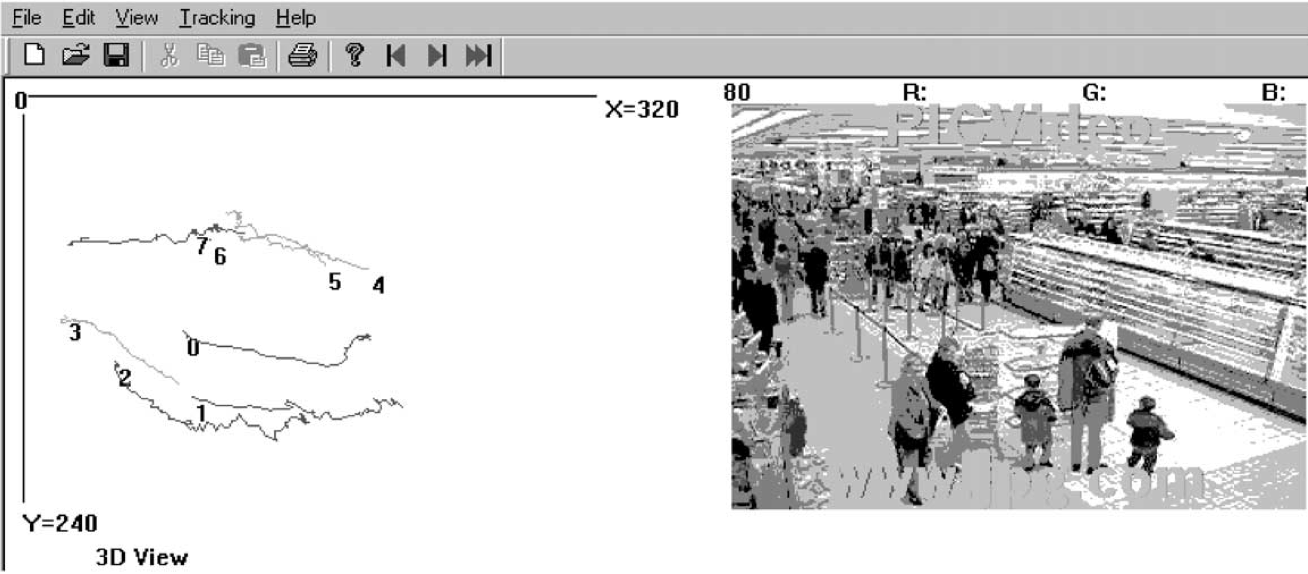
\includegraphics[width=\textwidth]{images/cctv_tracking_newman_pic1}
    \caption{Example of CCTV-based customer tracking from work by Newman et al~\cite{Newman2002253}}
    \label{fig:cctv_tracking}
\end{figure}


\section{Tracking using MAC address}
\label{sec:mac_tracking}

To see where a user has been and how he has moved, tracking system needs to be able to perform two operations. First, it needs to be able to determine the location of the device in question. Second, as the data is not continuous but comes with single, discrete points, all the location data needs to be linked together. That is, a device needs to be assigned some form of a unique ID.

Wireless nodes send their MAC address with every probe request, as we learnt in Section~\ref{subsec:active_scanning}. The MAC address is also globally unique; see Section~\ref{sec:MAC}. Therefore the MAC address seems to be a good candidate for an ID, so we can continue towards a much harder problem, actually locating the nodes.

\subsection{Determining the location of a node}
\label{sec:location}

A na{\"i}ve yet robust way to approximate user's location would be to look which AP received node's probe request. In Figure~\ref{fig:position_1} an oversimplified situation is presented: there is a rectangular-shaped building with a room, a few shelves, and four access points. The APs are labeled with letters from A to D. The building is divided into four sections, and the position of a mobile device is determined by looking which AP received a request from it. For example, it might be assumed that only AP D receives a signal from the mobile device in the picture, and therefore the user is somewhere in the lower-right section of the building.

\begin{figure}
    \label{fig:position_1}
    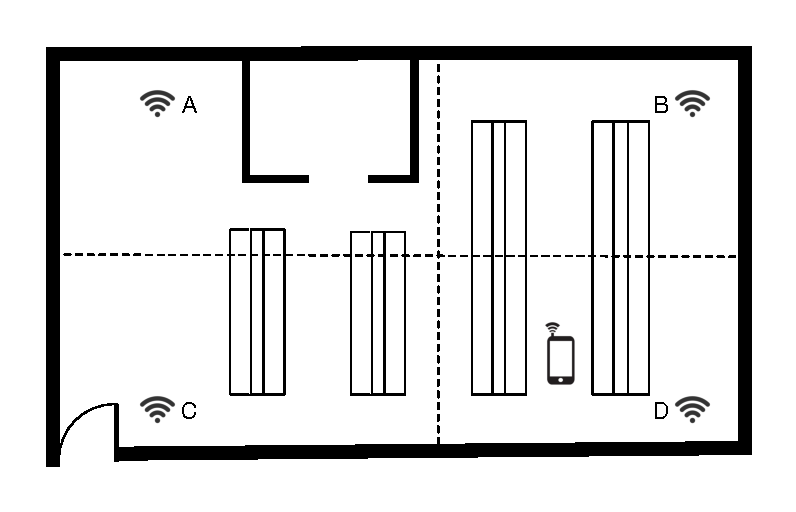
\includegraphics{images/positioning_1.pdf}
    \caption{Simplest way to achieve positioning}
\end{figure}

However, things are obviously not that simple. In real-life situations, coverage of a single AP can be large and easily overlap with others, and signal from the mobile device in Figure~\ref{fig:position_1} could also be in the ranges of APs B and C. A real-life example from~\cite{xiang2004} is presented in Figure~\ref{fig:ibm_coverage}, where in Figure~\ref{subfig:ibm_layout} the layout of building is presented, and in Figure~\ref{subfig:ibm_strength} the strength of a signal from a single AP is shown. Note that the whole floor is covered by the AP at least in some amount, but there are still four more APs. This suggests that at least in this case, a device can always catch more than one signal.

\begin{figure}
\begin{center}
\subfigure[Layout of the building]{
  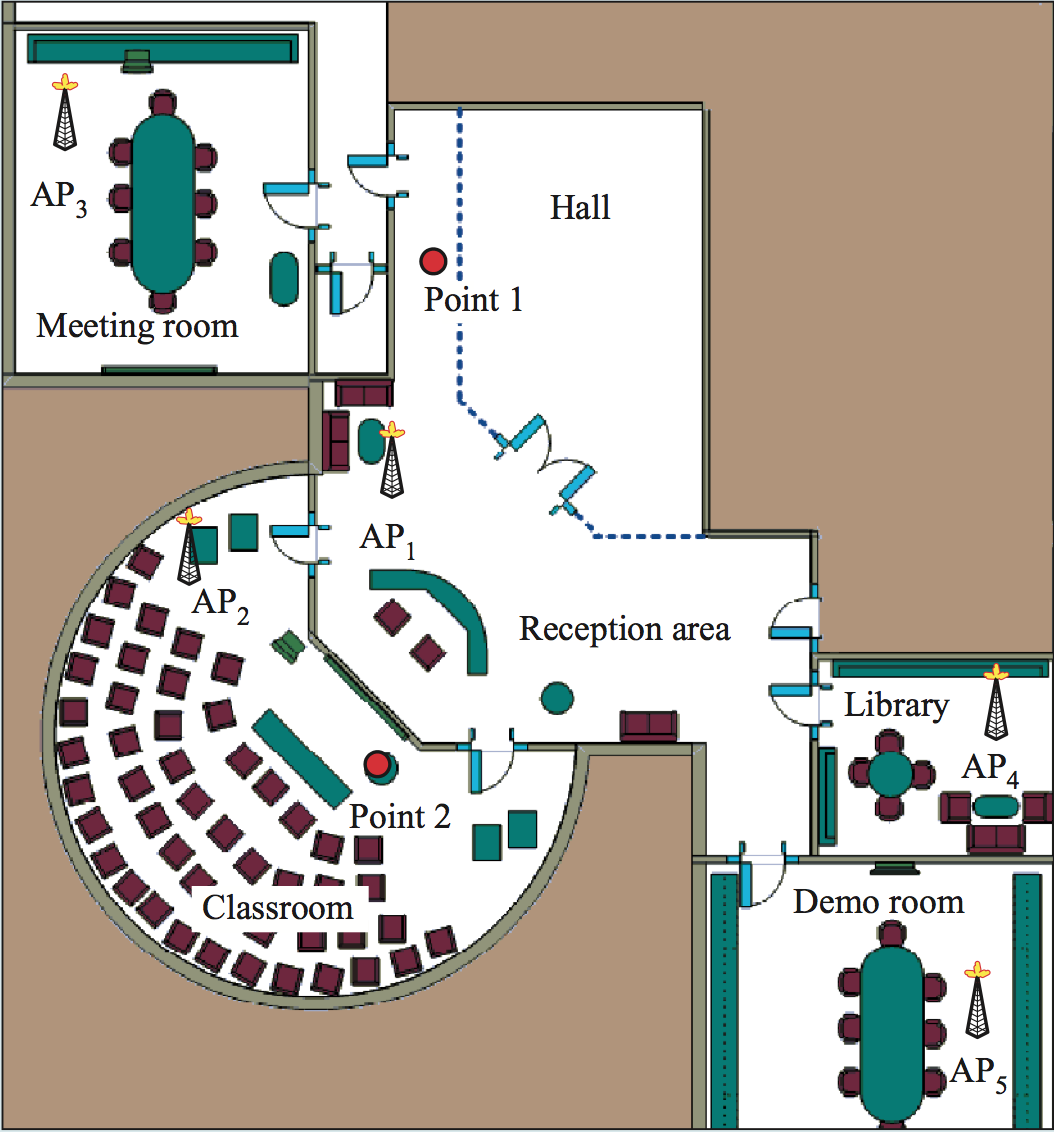
\includegraphics[scale=0.34]{images/ibm_wlan_layout.png}
  \label{subfig:ibm_layout}
}
\subfigure[Coverage of AP$_1$]{
  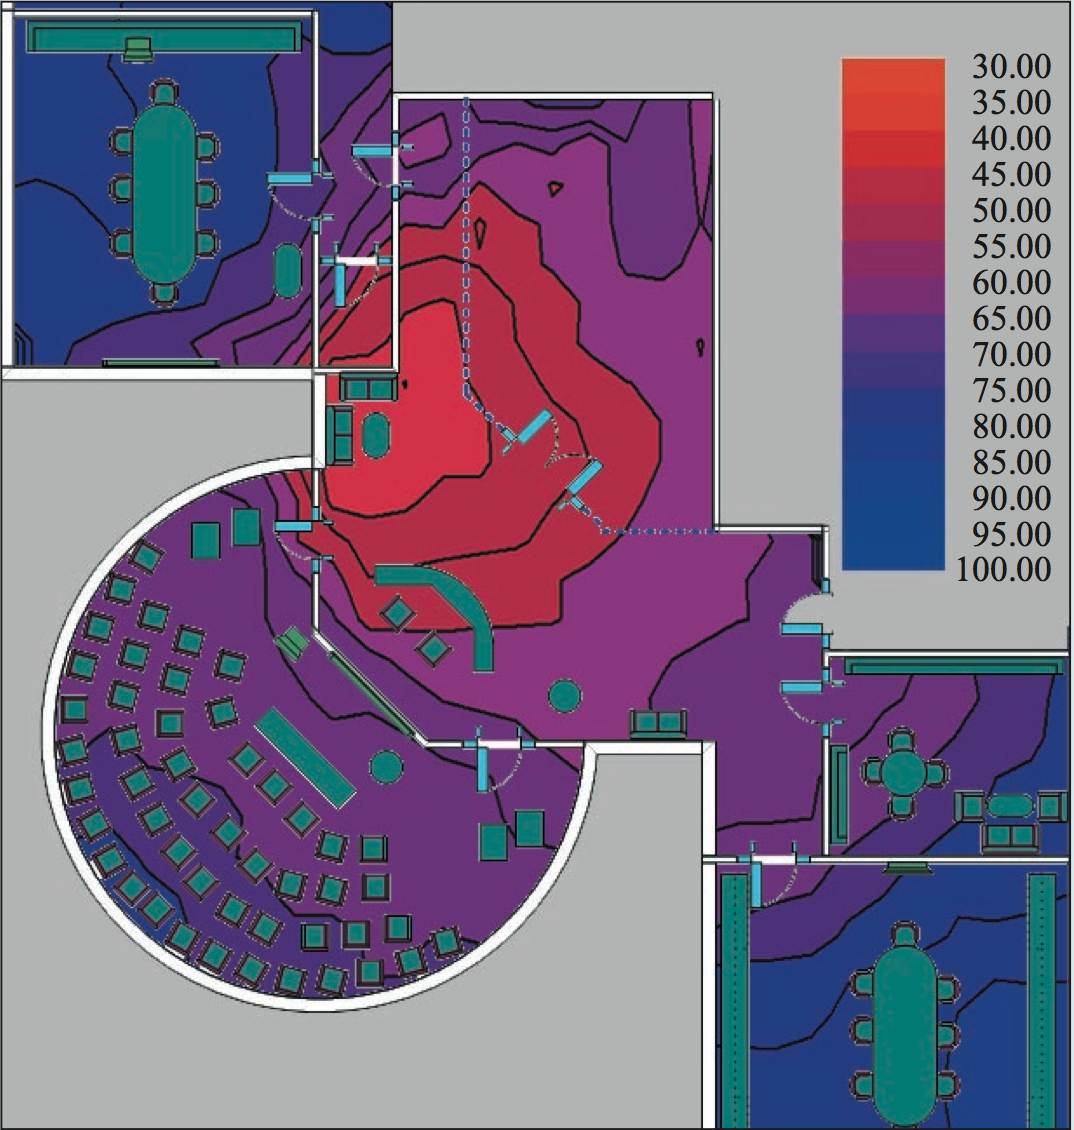
\includegraphics[scale=0.34]{images/ibm_wlan_strength.png}
  \label{subfig:ibm_strength}
}
\caption{A real-life example of WLAN coverage. Taken from~\cite{xiang2004}.}
\label{fig:ibm_coverage}
\end{center}
\end{figure}

Distance from a node to an AP can be estimated by using strength of received radio signal (RSSI, Received signal strength indication). This cannot give the exact distance, as transmitting power varies between devices, and we do not know the initial power. However, this problem does not prevent us from using it as an estimate, because we are interested in relative distances. Continuing the simple way, we can select an AP that received the strongest signal; for a little more accurate result, a triangular-based calculation could be done with simple trigonometry, if at least three APs received the signal.

We should keep in mind that all kinds of obstacles, such as walls, will reduce the accuracy of measurements. To obtain higher accuracy, lots of research has been done for creating WLAN-based positioning systems. This research includes more and more sophisticated methods for determining the location. Xiang et al.~\cite{xiang2004} constructed a model of signal propagation, Roos et al.~\cite{roos2002} used probablistics and machine learning, and so on. Most of this research tries to let mobile phone determine its own location based on the signal from APs, but exactly the same approach can be used other way around, as we would like to: to let AP find out mobile node's position by node's signals.

\section{Profiling users using SSIDs from active scanning}
\label{sec:ssid_profiling}

Whereas previous section discussed on possibilities to track a device based on MAC address, in this chapter we will see how it is possible to profile users who have left active scanning running on their devices. Later we conduct a practical study based on techniques presented in this chapter; this is done in Chapter~\ref{chapter:practical}. 

First we assume that a profiler has set up a device that collects all the probe requests sent by other devices. After that, the profiler looks for SSIDs included in probe requests and tries to figure out some information about customers based on the SSID data.

\subsection{Geolocation}
\label{subsec:ssid_geo}

SSIDs do not necessarily leak any information about their location. In some cases that may be true: for example, an open network in Aalto University is called ``Aalto open'', or a public network at Los Angeles airport as ``LAX-WiFi'', but in general no such connection can be drawn.

Numerous applications would benefit from ability to connect wireless network APs to their physical geolocation, or vice versa. For example, this could serve as a backup solution in lack of GPS signal for positioning, which is the case when user is inside a building. The same mapping other way around, mapping location to wireless access points, would allow mobile phone users to find a nearby open WLAN instead of consuming expensive cellular data transfer.

The solution for this problem is quite simple and straightforward. A collecting device goes around the world, capturing all the SSIDs and MAC addresses of WLANs it finds. Then, using GPS, it gets its own location, which serves as an estimate for the network location, and stores the data into a simple database. Numerous companies have already done this: the best-known case might be Google, who did it with its Street View cars~\cite{google_wifi_collection}. 

Another way to get the data is to use crowdsourcing -- in other words, to let users do it themselves. In this way, every time a user connects to a new network, exact geolocation is saved with phone's GPS receiver. The location, the SSID of the network, and probably more information such as signal strength are then saved into a database. Using this approach, data-collecting company can gather lots of data with relatively low expenses, and may be able to achieve higher accuracy compared to smaller dataset.

Both of above-explained applications for geolocation data of wireless networks have been implemented. Google uses WLAN locations with its Android operating system to provide location data based on networks it finds around~\cite{google_wifi_collection}. Nokia and Microsoft use same kind of data in Windows Phone in order to locate open WLANs near the user's own location~\cite{nokia_datasense}.

In addition to proprietary databases, there exists an open one called WiGLE, Wireless Geographic Logging Engine~\cite{wigle}. WiGLE has operated since 2001, and it provides almost 150 million unique Wi-Fi networks with location data (as in August 2014). WiGLE gets locations from users' submissions and gives data access for free. In itself, WiGLE is not suitable for large-scale analysis, because it does not provide full data dump and limits amount of queries one is able to perform daily. For this research, we have been temporarily granted higher limits.

It is important to note that the mapping from SSID to location is not one-to-one: multiple wireless networks around the world may share the same SSID. In fact, this is quite common, since many WLAN owners do not change the default SSID of their AP. In WiGLE, most common SSIDs are \texttt{linksys}, \texttt{NETGEAR}, and \texttt{dlink}, which all are default SSIDs of different AP manufacturers.

Some useful information can be obtained from geolocated SSIDs. The easiest one is to try to guess where the users might live by figuring out where the majority of SSIDs are located. Not exact results can be got with this approach, but city-wide accuracy should be possible in many cases.

Another interesting factor is to determine how much a user has traveled: people with SSIDs around the world might behave in a different way than ones with SSIDs from only one country. 

We can develop this approach further by trying to identify concrete places user has visited, for example hotels, restaurants, and universities. Categorizing places is possible with combining data from multiple sources and datasets, for example Expedia Hotel Database~\cite{expedia_hotel_db}, Yelp~\cite{yelp}, and Google Places~\cite{google_places}. Even more, Expedia provides some information of quality and price range of a hotel, and Yelp pricing scale for services, which can also be used to characterize a user: does he tend to use high-quality services or likes to prefer low-price alternatives?

\subsection{Discovering real-life relationships from common SSIDs}
\label{subsec:ssid_commons}

After collecting much of SSIDs from lots of devices, it is possible to discover friendships based on which SSIDs people share with each other. A paper on this approach has been written by Cunche et al. (2014)~\cite{cunche2014linking}

In the paper, they have two datasets: one collected from small number of volunteers with known friendships, and another from the wild, which has been collected over a six-month period in Sydney, Australia. The dataset of volunteers contained strong relationships, such as close friends and family members. Authors created a model based on observations of the known dataset and applied it to unknown data from the public.

Finding strongly connected nodes in two datasets has been studied well in computer science, so there are numerous mathematical methods developed for this particular problem. These methods are called similarity metrics, and the idea is to measure how similar two nodes are based on their feature set (here, list of SSIDs). 

A simple metric for comparing two samples is the Jaccard Index. It is defined as follows, where $X$ and $Y$ are two sets of SSIDs.

$$J(X,Y) = \left| \frac{X \cup Y}{X \cap Y} \right| $$

However, the Jaccard Index takes into account only the size of intersection, and not the fact how popular an element was in the dataset. It does not matter whether the two nodes had the most popular SSID, for example \texttt{linksys}, in common, or if they were the only two nodes that had the SSID \texttt{Super-Private-XYZ123-Network}. In the paper, Cunche et al. argue that having a rare SSID in common should yield for stronger possibility of relationship. That is a reasonable argument, especially when we consider the long tail of SSID frequency: a few SSIDs are extremely common, but huge majority of SSIDs appear only in one or two devices.

To take these characteristics of SSIDs into account, Cunche et al. develop a new metric, which is defined as 
$$\text{Psim-}q(X,Y) = \sum_{z \in X \cap Y} \frac{1}{f_z^q}$$
where q is a parameter and $f_z$ is the frequency of element $z$. The authors obtained best results when $q=3$.~\cite{cunche2014linking}

Probably the biggest problem for finding relationships in dataset is that it is computationally somewhat heavy. Complexity is $O(N^2)$ where $N$ is the number of devices in a dataset, so it may be impractical to try to find all the links in a very large dataset, such as Cunche's six months long range of data. Nonetheless, if we are limited to small population, for example people visiting a specific place, a store, or an airport during a day or week, it most likely is perfectly feasible to calculate all possible combinations.

% this is more for the next section
% Real-life use cases to benefit from such a findings can also be found. If we are not limited only to strong connections, such as family members, weaker connections can suggest that users share some charasteristics. After having categorized users in different clusters, one could try to look if the clusters are distinguishable from each others. For example, does the one group look like younger people, and do they visit the store on specific time of the day, or spend notably more or less time in the shop?

\subsection{Clustering}
\label{subsec:clustering}

To generalize previous idea, we can see the situation as a weighted graph. In the graph, mobile devices are nodes, and the edges represent the similarity of two nodes. More similiar nodes have an edge with greated weight; if two nodes have nothing in common, there is no edge between them.

Once again, the simplest method to create similarity function are calculating the size of intersection of SSID lists or the Jaccard index. We can also use advanced algorithms, such as Psim-q.

When we have formed a graph, we can search try to search for clusters. There is no single, widely-accepted definition for a cluster in graph~\cite{schaeffer2007graph} , but we will define it informally as ``recognizing natural groups within a class of entities''~\cite{van2000graph}, or partitioning the graph in groups in a way that distance inside a cluster is low and distance between clusters is high. Therefore, we are trying to look for groups of nodes that have common charasterics. The difference to previous section is that there we searched for strong connections between two nodes; now the size of group is larger than two.

Finding the clusters in the graph is therefore our actual problem. Luckily, we do not need to invent our own algorithm, since this is a general graph problem, and it has been studied in computer science before.

A possible algorithm could be \emph{hierarchical clustering}~\cite{schaeffer2007graph}. Here, the idea is to build a tree of hierarchy. Depending of particular algorithm, the process can start from top or bottom of hierarchy. In top-down (``divisive'') algorithms, initially every node belongs to a single cluster, and in every step clusters may be split into two new clusters. In bottom-up approach (``agglomerative''), every node is initially its own cluster, and in every step they may be merged with others. When specific stopping condition is met, the algorithm terminates, or it can build the whole tree and select the best point to break dataset into clusters, so-called \emph{knee point}. For this, there are numerous methods available, including largest difference between two points, largest ratio between two points and so on~\cite{salvador2004determining}.

Generic hierarchical clustering has time complexity of $O(N^3)$~\cite{manning2008introduction}, which may be problematic for very large datasets, but most likely usable for us. The algorithm does not require us to provide number of clusters beforehand, which is a useful feature: we do not now the structure of data before finding clusters. It is also easy to understand and relatively simple to implement, and may reveal interesting facts about the structure of data.

Another promising approach could be \emph{Markov Cluster Process} (MCL Process), introduced in van Dongen's PhD dissertation (2000)~\cite{van2000graph} and taught nowadays in university classes~\cite{mlc_macropol}. The algorithm first transforms a graph into a transition matrix, where element $(x,y)$ denotes the weight from $x$ to $y$. Columns are normalized so that each sums to one. After that, there are two operations: expansion and inflation. Expansion simply raises the matrix to power of $e$, which is a parameter. Inflation consists of squaring every column and then normalizing it again to sum to one; this way, inflation strengthens already strong connections and weakens already weak ones. In other words, expansion allows flow to connect new parts of the graph and inflation grows the range of values. Inflation and expansion are repeated until the algorithm convergences. Resulting matrix gives the clusters.

MCL has same kind of problems than hierarchical clustering. First, MCL's time complexity is $O(N^3)$, where $N$ is number of edges, which may become a problem with very large graphs. However, for our use it most likely is manageable, as numbers of nodes is closer to thousands than millions. Second, it cannot find overlapping clusters -- each node belongs only to one cluster. However, by providing different initial parameters for multiple runs, we may be able to retrieve different clustering results.

As we have seen, both algorithms suffer from inability to deal with overlapping clusters. Finding clusters that can overlap is an open research question, with some algorithms proposed in last years, for example OClustR~\cite{PerezSuarez2013234} and DClustR~\cite{PerezSuarez20133040} from P\`{e}rez-Su\'{a}rez et al., and another link clustering based method by Shi et al.~\cite{Shi2013394}. Development of efficient algorithms is still ongoing.


\subsection{Social media networks}
\label{subsec:social_media}

A novel and interesting approach is to combine SSID data with social media. In this section we will present the idea, and in Chapter~\ref{chapter:practical} we will perform practical experiment to see if the idea can be implemented with our resources.

The key idea and goal of our research is to find the owner of a device from social media based on SSID findings. Possible social media platforms include Facebook, Twitter, Foursquare, Google+ and others. These include --- or at least provide a possibility to include --- a location data into a posting. 

Thus, we have three datasets. First, we have collection of SSIDs from target's device. Second, we have a mapping from SSID to geolocation. Third, we have a database of people's social media postings with their locations. By combining all of them, we may be able to reveal the social media profile used by the device user.

From the social media service list above, Twitter can be considered the most public. By default, every \emph{tweet}, a post to Twitter, is visible to everyone, whereas in Facebook the default audience is limited to user's friend network. For this reason, we will study primarily Twitter, but other networks share the same idea, if private access to the database is granted.

Twitter provides a free-of-charge application programming interface (API) to its data.~\cite{twitterapi} Using the API, one can fetch tweets with or without specific search criteria. One possible method to filter the results is by location coordinates.

As a drawback, searching by geolocation is limited to 180 requests in an hour. Also, only recent tweets are available. Nevertheless, the idea does not suffer from these limitations, as we should assume that a private API or future development will allow access to larger amount of data. Possible problems may also arise from the fact that not every posting contain location information.


\subsection{Semantic SSID analysis}

Semantic SSID analysis is a technique where we try to profile a user based on the content of information retrieved from SSIDs. This is a technique that is obviously possible to some extent, but to our knowledge no studies have actually tried to implement it.

In semantic analysis, we know beforehand what we are looking for. In graph-based clustering explained previously, we have only data and try to find anomalies within it.

We see at least the following possibilities:\\

\textbf{Detect price scale of services used.} Yelp~\cite{yelp} provides price range in a scale from 1 to 4. Using it we might see if user tends to use low-price services or high-end ones.

\textbf{Identify students and other academic people.} Universities usually have their own wireless networks, individual ones or common \emph{eduroam} in Europe, so they are easy to spot.

\textbf{How much is a user traveling?} Identify airports and hotels. Categorize user to different price categories based on hotel's average price level. Probably same kind of information can be extracted from restaurants' and cafes' names.

\textbf{Distuingish between locals and foreigners.} If the user has locations only nearby, he is probably a local. If majority of locations is from somewhere else but within a reasonably small radius, that might be his home location. However, making reliable difference between someone's hometown and a place where he has visited might be difficult.

\textbf{Monitoring behavior in a specific industry.} We can characterize user's behavior in some industries, where wireless networks are common. For example, many hotels offer a network. Hotel owner could look for his customers history: have they visited a lot competitor's hotels, or is this even the first hotel visit they have? 

\section{Other information obtained from probe requests}
\label{sec:other_info}

We are able to find even more information from probe requests than we have discovered so far. As discussed in Section~\ref{sec:MAC}, first half of a MAC address, Organizationally Unique Identifier (OUI), is determined by manufacturing company. When comparing that to a database containing all the OUIs assigned, we will be able to discover the manufacturer of a node. The database is available for free~\cite{oui_listing}.

In~\cite{pang2007802}, Pang et al. have been trying to fingerprint WLAN users by different traffic characteristics. The methods they used were (1) network destinations, (2) SSID probes, (3) broadcast packet sizes, and (4) MAC protocol fields. 

However, their approach was different from ours, as they study a scenario where analyzer can monitor all the traffic: the user has connected to a wireless network run by analyzer. In our work, we are limited to the probing phase, which happens before any connection has been made. This limitation rules the first method, examining network destinations, out. Also, SSID probes are already covered elsewhere in this work.

Broadcast packet sizes are a possible approach. Some services and applications broadcast information or advertisements about themselves. For example, Dropbox, a cloud-storage service provider, has a desktop app that tries to find computers with linked Dropbox accounts in the local network. If they were found, transferring data between them would be a lot faster and cheaper than via public internet.~\cite{dropboxlan} All the content of broadcasts are encrypted in secure WLANs, but broadcasted packets can still be found, because they are sent to a known broadcast MAC address \texttt{ff:ff:ff:ff:ff:ff}, and the MAC address is always sent in plaintext. The size of the packets is also unencrypted, which leaves the possibility to retrieve information even from encrypted networks.

The last method, MAC protocol fields, tries to exploit the fact that MAC header includes flags and fields that vary between different manufacturers and configurations. As Pang et al. themselves note, this is usually not enough to distinguish users uniquely, because quite a many people use exactly the same model of a device. However, this method can be used in addition to others, if necessary.

It should be noted that both of these methods are not likely to work in our case. Broadcast packets are sent only when user has already joined a network, and we are studying the situation where user is still probing for available alternatives. MAC protocol fields are only a small piece of information, and those fields do not differentiate devices enough.

\subsection{Wi-Fi Protected Setup}
\label{sec:wps}

Another exploitable feature is Wi-Fi Protected Setup (WPS). The technology is used to ease the setup of a secure, consumer-grade wireless network. Using WPS, users do not need to know about technical details or enter complex passwords to gain access to WLAN, but instead can push a button on both AP and their mobile device. There are also another ways to implement the standard, including entering PIN code or using NFC-capable device.~\cite{alliance2007wi}

The actual standard for WPS is available without a charge only for Wi-Fi Alliance members~\cite{alliance2007wi}, but we do not consider that as a constructive way to develop technical standards. Therefore we resort to reverse engineering the standard using packet analyzing tool called Wireshark~\cite{wireshark}, which has implemented the WPS protocol. Wireshark is open source software, so the protocol can be analyzed with a low enough effort by reading source code and running analysis on captured packets. Also, there are other documents freely available to gather information about the protocol, such as Microsoft's technical specification of WPS inside their own document~\cite{microsoftWCN}.

In the protocol there are three actors: enrollee, AP and registrar. Enrollee is a user willing to join a wireless network using WPS. Registrar is the authority who will gain or deny access. AP is the same access point as previously, but this time it is specified to act as a link between enrollee and registrar. In practice, and especially in consumer-grade devices, registrar's functionality is often included in AP. 

\begin{figure}
    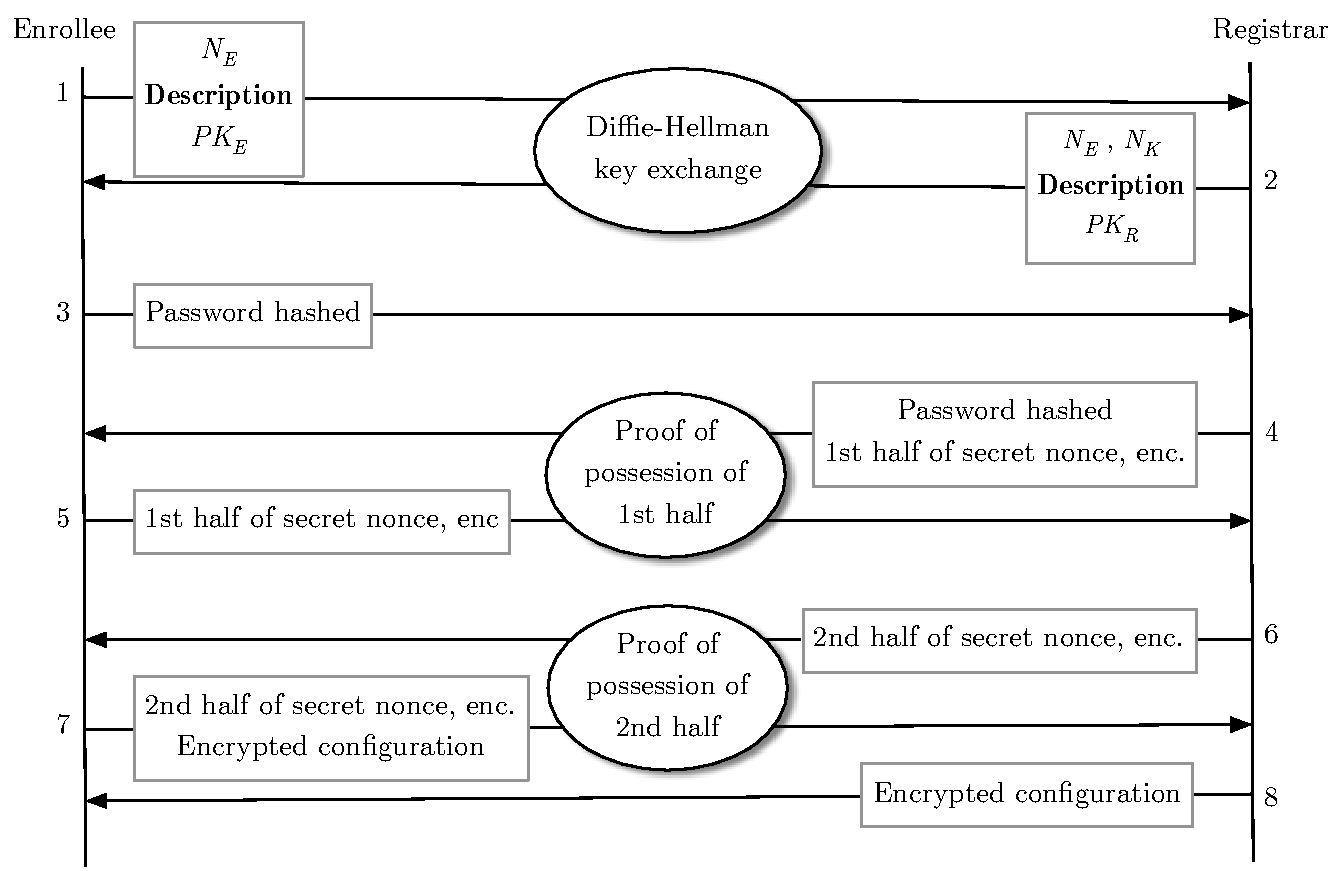
\includegraphics[width=\textwidth]{images/wps}
    \caption{Protocol for joining a WPS-enabled WLAN. Simplified from~\cite{microsoftWCN}}.
    \label{tab:wps}
\end{figure}

Because joining a WPS-enabled network has been wanted to make easy but secure for end-users, it is somewhat complex in technical side. Simplified version of protocol is shown in Figure~\ref{tab:wps}. Basically, first enrollee sends its nonce, its own description and its public key to registrar, and registrar replies with the same kind of message with its own information. Then, in messages 3 and 4, parties make precommitments that they know the password by sending it in hashed form. In messages 4-7, parties send their own secret, encrypted hashes, which can be used with previously-sent hashes to make sure that the password was correct. Finally, in message 8, registrar sends WLAN configuration data including credentials to join the WLAN.

The most important and interesting part for us is in the very beginning, since we are interested in probe requests. We found that some devices are actively sending WPS requests hoping that an AP would reply. This request is the same as message 1 in the protocol, and it is sent in a probe request frame's last field, targeted for vendor-specific information.

In message 1, there is a broadly-named field ``Description''. The data it includes makes it worth to look closer. Microsoft's document says that it is ``[a] human-readable description of the sending device (UUID, manufacturer, model number, MAC address, and so on) and device capabilities such as supported algorithms, I/O channels, and Registration Protocol role.'', and Wireshark confirms exactly that. Also, there is a field called ``DEVICE\_NAME'', which is the human-readable name user has given to his device, for instance ``Pekko's phone''.

With all this information, we may be able to
\begin{enumerate}
    \item categorize users by their phone manufacturer and model,
    \item identify a node with UUID in addition to MAC address, and
    \item possibly extract private information from user, for example user's real name from device's name
\end{enumerate}


% this may be left out
% \section{Evaluation of current mobile devices}
% \label{subsec:evaluation}
% iphone, android, WP
% do they broadcast all the ssids or just a wildcard?
% order? SEE THE SOURCE CODE!


%%%%%%%%%%%%%%%%%%%%%%%%%%%%%%%%%%%%%%%%%%%%%%%%%%%%%%%%%%%%%%%%%%%%%%%%%%%%%%%


\chapter{Active man-in-the-middle attacks}
\label{chapter:attacks}

In addition to passive surveillance, there is a possibility for performing active attacks against users. In active attacks, the attacker does not only monitor user's behavior, but instead sends malicious packets to perform desired activities. 

All the following attacks are some variants of man-in-the-middle (MITM) scheme. In MITM attack, the attacker positions himself between user and the service user is connecting to. This way, an attacker is able to read and alter all unencrypted communication while remaining transparent to the victim. The following attacks differ by how an attacker gains such a position.

\section{Unencrypted access point}
\label{sec:attack_unencrypted}

The easiest attack is to set up an unencrypted access point and monitor all the traffic that goes through it. Obviously this is not very sophisticated, but at least some users are likely to be tricked into this one for various reasons.

First, they do not know or care about wireless network security but only see a free connection to internet to use. No technical security measure on link layer can save users, if they want to use an open connection with unknown administrator.

Second, multiple versions of Windows have a feature to join any unsecured wireless network in the range~\cite{dai2005attacking,windows_wifi_answers}. Therefore, user's computer can join an open network without user being aware of that. Even worse, with some versions of Intel wireless drivers, the setting to disable the automatically-connecting feature is hidden elsewhere than in unusual settings dialog, making it difficult to disable even for little more experienced users.~\cite{windows_wifi_answers}

An unwanted connection can be damaging, even if the user realizes the mistake relatively fast and disconnects his computer from the open network. Quite a many services want to synchronize their data right after connected; for example, an email client would like to get new messages immediately when the client device becomes online. Therefore it is certainly possible that user's credentials are sent and exposed during first moments in a new network.

\section{Evil twin}
\label{sec:evil_twin}

If there are multiple alternatives available, nodes have a couple of methods to decide which network they join. In Windows, there is a preferred wireless networks list, which specifies the order in which computer should connect to networks~\cite{windows_wifi_preferred}. 

If there is no preferred networks available, a node may choose the one which has the strongest signal strength -- or if not choose, at least present it as a first alternative to user. Another methods have also been proposed, such as testing networks for their bandwidth and choosing the best~\cite{Nicholson:2006:APselection}. However, these kinds of advanced methods have not yet been implemented, so previously-selected networks and physical-layer signal strength are the most common criteria used nowadays.

\begin{figure}
    \begin{center}
    \subfigure[Normal scenario]{
      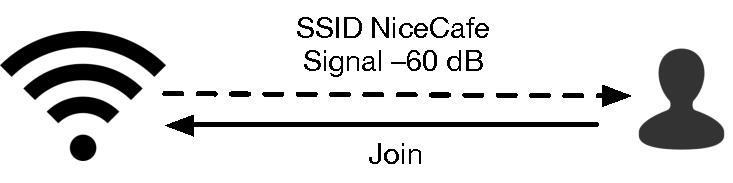
\includegraphics[width=0.6\textwidth]{images/evil_twin_normal.pdf}
      \label{subfig:evil_twin_normal}
    }
    \subfigure[Evil twin steals the connection with the same SSID]{
      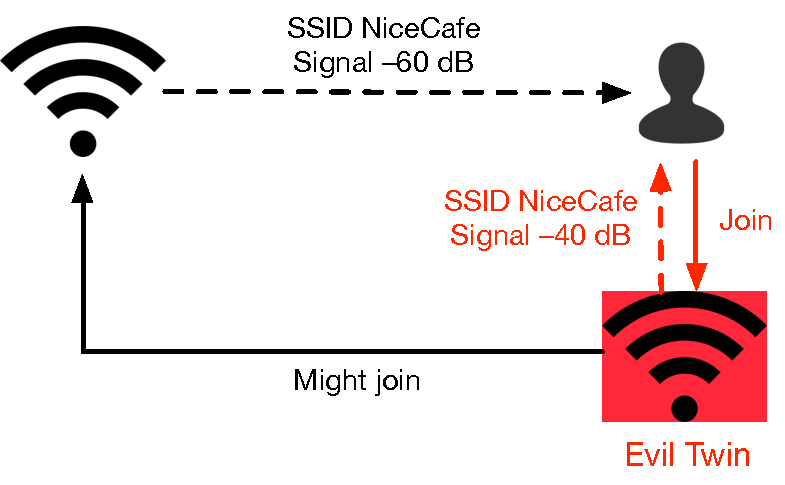
\includegraphics[width=0.6\textwidth]{images/evil_twin_mitm.pdf}
      \label{subfig:evil_twin_mitm}
    }
    \caption{Evil twin attack}
    \label{fig:evil_twin}
    \end{center}
\end{figure}

The idea of an evil twin attack is presented in Figure~\ref{fig:evil_twin}. First, there is a normal scenario. A user is having a coffee in his favorite cafe, and joins cafe's open, unencrypted network which has an SSID \texttt{NiceCafe}. Everything goes well. The next time the same user is visiting the cafe again, but this time there is a malicious access point with the same SSID, \texttt{NiceCafe}. Remember, SSID is not a unique identifier, and it can be chosen freely. The malicious AP is located closer to the user or has a more powerful antenna, so its signal is much stronger than the original AP's. Therefore, the user connects to the malicious access point, and all the traffic is suddenly exposed to the attacker.

Evil twin can appear also in another place than original AP was. The attacker can set up an AP with SSID ``Starbucks'' even if there is no Starbucks nearby: the user may not notice the problem, if his computer connects automatically to the network.

\section{Man in the middle exploiting WLAN probes}
\label{sec:mitm_probes}

In previous section, an attacker knew beforehand that there was a specific network available and chose his SSID based on that. This is not necessary, and opens room for a more powerful attack.

A rogue access point can be listening for all the probes in the air. When it sees something, for example a node probing for a network \texttt{NiceCafe}, the AP can pretend that its SSID is \texttt{NiceCafe} and let the node to connect.

If a node is not probing any specific SSID but asking all the nodes to broadcast theirs, the basic version of this attack will not obviously work. Still, there exists an opportunity: quite a many device has at one time connected to a network with an unchanged, manufacturer-default SSID, such as \texttt{Linksys} or \texttt{dlink}. According to WiGLE~\cite{wigle}, five most common SSIDs account for 4.2~\% of total SSIDs seen, and 100 most common SSIDs for 12.7~\% of total. An attacker could try all the common ones and hope that at least one of them is in node's SSID list.

\section{Encryption}
\label{sec:attack_encryption}

A particular problem for attackers is encryption. Wireless networks may be secured using techniques such as WPA2 (Wi-Fi Protected Access 2), which is based on a pre-shared secret -- a passphrase. Both parties of communication, client and AP, identify each other using four-way handshake, so the AP cannot only wait for client to send a passphrase and record it. Since the attacker does not know the passphrase and it is not included anywhere in cleartext, WPA2 renders previous attack useless.

Another possible piece of encryption is Transport Layer Security, TLS (predecessor known as SSL, Secure Sockets Layer, and often these two are mixed). With a bit confusion with the name, it can be said that TLS is implemented between transport layer and application layer. As this layer is above link-layer, on which attacker operates, it should be a safe alternative.

However, there is a technique called sslstrip~\cite{marlinspike2009new}, which is designed specifically to redirect badly implemented TLS/SSL connections to unencrypted ones. At this time, using TLS can be considered only a partial solution against MITM attacks: the technique is safe only if used correctly, which is not always the case.

\section{Existing software and devices}

\begin{figure}
    \center
    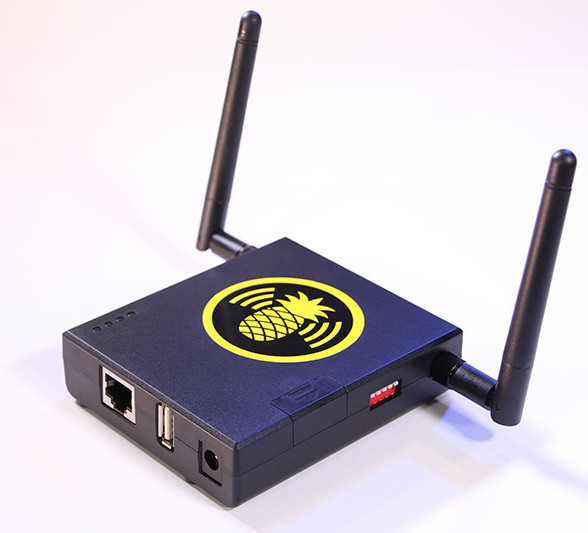
\includegraphics[width=0.8\textwidth]{images/wifi_pineapple_pic}
    \caption{WiFi Pineapple, a ready-to-use toolkit to conduct attacks against wirelss networks. Note the size: there are an RJ45 and an USB port visible for comparison.}
    \label{wifi_pineapple_pic}
\end{figure}

Concepts discussed here are not new, and for them there are specific tools implemented.

In previous section we mentioned technique called sslstrip; to prove its efficiency, authors decided to publish fully-working tool that implements the attack. The tool is available to everyone.~\cite{marlinspike2009new}

Most comprehensive and most easy-to-obtain toolkit is WiFi Pineapple~\cite{wifipineapple}. It includes numerous tools for MITM and other attacks and sells for as low as \$~100 (as in August 2014). The device is shown in Figure~\ref{wifi_pineapple_pic}, where especially noteworthy is its small size, 10 x 8 x 3 cm. In the picture, there are RJ45 and USB ports visible, so that one can feel its small size.

With these kinds of ready-made tools, performing MITM attacks are totally feasible with only a little knowledge and skills, and they must be taken seriously.

%%%%%%%%%%%%%%%%%%%%%%%%%%%%%%%%%%%%%%%%%%%%%%%%%%%%%%%%%%%%%%%%%%%%%%%%%%%%%%%


\chapter{Legal status}
\label{chapter:legal}

So far we have seen how it is possible to collect data from mobile devices, how to interpret the collected data, and how to perform active attacks exploiting features of said devices. In this chapter, we study the legal framework of the issue.

Most of the cases have basis on privacy legislation. Privacy is recognized internationally on the Universal Declaration of Human Rights~\cite{udhr}, but actual laws are not universal but vary greatly between countries. Thus, we concentrate on two major players in the field, the United States and the European Union.

We will divide our study in three parts:
\begin{enumerate}
    \item Is collecting SSIDs from access points and mapping them legal, or how it is regulated?
    \item Is collecting SSIDs from mobile devices legal, or how it is regulated?
    \item Is analyzing the SSID data legal, or how is it regulated?
\end{enumerate}

Active man-in-the-middle attacks are analogous to wiretapping phone communications, which is illegal by well-established laws on wiretapping, secrecy of letters, and secrecy of communications. Thus, we are not interested in them and will not study those.

The best-known and best-documented legal case for two first questions is Google's Street view, on which we give small background information before we begin. After the study of current regulations, we will look for the ongoing development in the field and discuss the situation.

% is there any legislation? terms and conditions -- can't apply, if the user hasn't joined a network

% approaches to get an ``I agree'' from customers: 
% (1) put a physical sign (case Nordstrom, Inc) 
% (2) use a specific app (case Helsinki-vantaa)
%     -> if an app requires Wi-Fi permissions (on android), it can look easily for all previous networks (there was a paper on that)~\cite{2014_WISEC_Achara}

\section{Background of Google Street View case}
\label{sec:streetview}

The case with Google's Street View data collection has been a major case in terms of regulation of the topic, so we will first look on that. 

Steet View~\cite{googlestreetview} is Google's service built on their Maps platform. In Street View, one can view panorama photos taken from the streets. Google has collected the images by driving on streets with a car equipped with multiple cameras and a GPS device~\cite{streetview_behindscenes}.

Cars were collecting more information than only pictures of the streets. Google first told that they were collecting photos, WLAN network information including only access points' SSIDs and MAC addresses, and 3-D geometry data with lasers, all of them to help Google build location services. Google stated explicitly that it does not collect any payload information from wireless networks.~\cite{fleischer_datacollected,google_wifi_collection} However, that was proved false when German Data Protection Authority (DPA) wanted to audit the data, and Google admitted that it ``had mistakenly included code in our software that collected samples of payload data from WiFi networks''~\cite{eustace_datacollected}.

\section{European Union}
\label{sec:legal_europe}

Europe is a complex legal entity, as traditionally diverse countries are trying to harmonize their legislation inside the European Union. We concentrate on current status and forthcoming efforts of the EU and do not study minor differences or historical laws in European countries.

The EU can impose four different types of legislation:~\cite{lisbon_288}
\begin{description}
     \item[Regulation] becomes a law in every EU country without alterations.
     \item[Directive] is binding to every member state, but each of them will consider how to adopt it in the best way, taking into account their current laws.
     \item[Decisions] are binding but only to whom they are addressed.
     \item[Recommendations] are, as the name suggests, only opinions without binding force.
\end{description}

Legislation is created by the European Parliament, the Council of the European Union and the European Commission.~\cite{eu_institutions}

For privacy issues, there is European Data Protection Supervisor (EDPS), who works together with each state's Data Protection Authorities (DPA). With the European Commission, these institutions form \emph{Article 29 Working Party},~\cite{wp29_rules} which we will refer as \emph{Working Party}. The Working Party has only advisory status~\cite{wp29_rules}, but its opinions must be taken seriously, as it is in direct interaction with law-making institutes of the EU.

\subsection{Personal data}
\label{subsec:eu:personal_data}

According to the official opinion of the Working Party~\cite{wp29_185}, the relevant piece of legistation is the Data Protection Directive (1995/46/EC)~\cite{data_protection}. It states in the first article for its object that

\begin{quote}
    In accordance with this Directive, Member States shall protect the fundamental rights and freedoms of natural persons, and in particular their right to privacy with respect to the processing of personal data.
\end{quote}

The question therefore is (1) is mapping of WLAN access points ``personal data'', and if yes, (2) what consequences does it have in respect to ``protecting privacy''? Personal data is defined in Article 2(a) as

\begin{quote}
    any information relating to an identified or identifiable natural person ('data subject'); an identifiable person is one who can be identified, directly or indirectly, in particular by reference to an identification number or to one or more factors specific to his physical, physiological, mental, economic, cultural or social identity;
\end{quote}

Thus, the first requirement of personal data is that a person can be identified from the data. This interpreation is backed by an opinion on personal data by the Working Party~\cite{wp29_136}. In the opinion, there is an example saying that ``Images of individuals captured by a video surveillance system can be personal data \textbf{to the extent that the individuals are recognizable}.'' (emphasis added)

To recognize only a possible group of people is not enough.~\cite{wp29_136} For example, only the last name of an individual is not personal data when talking about the whole population of a country, but within a school class, the last name is enough to identify a single person, and therefore personal data.

Together with previous observation, we can note that identifying a group from big mass is not personal data, but multiple such identifications in a combination can result in personal data. Using the same example, one cannot identify a person when given only the class he studies in nor when given only his last name, but in a combination, identification is certainly possible.

If the data is considered to be personal data, there are numerous regulations that apply. Precise implementation is left for individual states, but they include at least
\begin{itemize}
    \item the data subject [target] must have given his consent, or there is a strong necessity such as legal obligation
    \item the data subject has to be given a permission to view or erase data about him
    \item the controller [collector of data] must implement measures to protect the personal data
    \item the controller must name a person who is responsible for ensuring data protection legislation in the organization
    \item in some cases the controller must notify local data protection authority
\end{itemize}

These requrirements would increase the costs, reduce effectivity, and sometimes render data collection almost impossible. For example, it would be extremely difficult for Google to get consent from everyone to collect their network's SSID. Also, requiring users to turn off wireless connectivity if they do not want to participate would not be enough, as the Working Party notes~\cite{wp29_185}:
\begin{quote}
    If the default settings of an operating system would allow for the transmission of location data, a lack of intervention by its users should not be mistaken for freely given consent.
\end{quote}


\subsection{Collecting access point data}
\label{subsec:eu_collect}

Next we will look for legal issues in collecting data from wireless access points in the European Union. We assume that a service is collecting two different pieces of data: SSID and location.

To make it easier, we first examine the case of collecting only SSIDs. SSIDs are names of networks, decided by network administrators. Clearly SSIDs of public networks, such as the ones in buses or schools, are not personal data. In private home networks they are difficult to categorize as personal data: in many cases, the SSID is the default (for instance, \texttt{linksys}) or an arbitary name (\texttt{My little network}). Also, SSIDs are not unique, and there are lots of networks with the same name. The only possibility to render a SSID for personal data would be if someone named his network after his own name (\texttt{John Doe's network}), but this happens really rarely --- in our study, we found 20 this kind of SSIDs out of 8,500, which is 0.2~\%. Also, this does not make any difference between owner and user of the network. Therefore collecting only SSIDs should not be treated as personal data.

Combining the SSIDs with location data raises more questions. If we know the location of an access point, can we link it to a specific individual? The first thing to note is that location data is only an approximation. The location of a collecting device is not the same as the location of access point, and in fact, even the location data of a collecting device may have errors. In rural areas where spaces between houses are large, it is certainly possible to map a single access point to a specific house; in dense areas such as cities, this causes problems and at least requires significant amount of manual work.

However, there are a couple of cases where precise identification could be possible. We have examined that some SSIDs include the first name of a person, such as \texttt{John's home network}. Given with an approximate location, it might be possible to say ``within this building, there is only one John, so the network is his''. 

The question whether SSID-location combination of data is personal data is therefore a question of reasonability of an event described above, and amount of work that is required to discover an individual: if identifying is theoretically possible, is it enough, or should it be easy enough for an average person to perform? The phrasing in the directive is the following~\cite{data_protection}:

\begin{quote}
    to determine whether a person is identifiable, account should be taken of all the means likely reasonably to be used either by the controller or by any other person to identify the said person
\end{quote}

This is a difficult question: what are ``all the means likely reasonably to be used''?. The Working Party notes that not only today's situation is enough to consider, but that also future development should be taken into account, if data is to be stored for longer period.~\cite{wp29_136} Because there have been no legal cases for the issue, we cannot answer this question reliably.

The Working Party has said in a different opinion~\cite{wp29_185} that 
\begin{quote}
    the combination of a MAC address of a WiFi access point with its calculated location, should be treated as personal data.
\end{quote}

However, in our case we had only a MAC address and an SSID, not the BSSID that would uniquely identify the access point. In an article written by Watts, Brunger, and Shires~\cite{watts2011european} authors argue that the practical likelihood of mapping an access point to an individual is extremily low, and therefore mapping of access points should not be treated as personal data, even when BSSID is collected. It is worth to note that the writers of the article were assisting Google on its Street View case, so their opinion is likely to be in favor of Google and against regulation of such databases.

Together with the Data Protection Directive, there is another possible directive for the case, the E-Privacy Directive (2002/58/EC). However, it is not relevant for the case. First, in the opinion of the Working Party, it is said to apply only to location data processed by telecom operators~\cite{wp29_185}. That can be read from the directive, where ``location data'' is defined in Article 2(c) as

\begin{quote}
    location data means any data processed in an electronic communications network or by an electronic communications service, indicating the geographic position [..]
\end{quote} 

SSID data from nodes or access points is not processed in electronic communications network or service, as they refer to telecom operators. This directive is therefore designed to protect privacy of cell-location data from mobile phones.

\subsection{Collecting node data}

The legal view of collecting mobile devices' data is analyzed in the same way as collecting AP data. An important difference is that one device is highly linked to an individual, whereas many people may use the same access point.

Every mobile device has an MAC address, which is a unique identifier. By tracking the movements of a person based on MAC address, and combining it with, for example, a CCTV camera, one may reasonably be able to identify an individual. This kind of information should be treated as personal data.

Case of collecting SSID data is a little more difficult. In fact, our experiment in Chapter~\ref{chapter:practical} deals with this issue, as we try to show what kind of data can be extracted from SSIDs. Therefore the question wheteher SSIDs are considered to be personal data depends highly on iterpretation of result like our study: is it considered reasonably enough? At least there is a possibility that SSID queries should be treated as personal data.

\subsection{Analyzing the data}

The analyzing phase depends greatly on the decision whether data collected is considered to be personal data or not. 

If it is, then all purposes of where data is used must have been told to the data subject -- that is, the target of collection -- beforehand, and his constent must be obtained. Also, there is so-called ``right to be forgotten'', which includes a possibility for everyone to see their personal data and ask for its deletion in the Data Protection Directive, Article 12~\cite{data_protection}. 

However, if the data is not considered to be personal data, no EU-wide legislation applies. 


\section{The United States}

The legal system in the United States is somewhat different from Europe. American Common Law is based on previous cases, and we will study Google's Street View case in detail, since it fits best in our topic.

\subsection{Collecting SSID data}
\label{subsec:us_collecting}

The relevant legislation for examining SSID data collection is the Wiretap Act~\cite{wiretap_act}. In \textsection 2511(1)(a) is clearly stated that

\begin{quote}
    any person who intentionally intercepts, endeavors to intercept, or procures any other person to intercept or endeavor to intercept, any wire, oral, or electronic communication [..] shall be punished [..]
\end{quote}

First question is on which parts of WLAN conncetion are included in ``electronic communication''. Visiting web pages or reading emails is definetely electronic communication, but SSID broadcasts are more problematic. In a case U.S. v. Forrester~\cite{us_forrester} the government had monitored Forrester's internet activity. In the decision of Court of Appeals, 9th Circuit\footnote{Court of Appeals, 9th Circuit is a federal court, which handles appeals from the western part of the U.S. There are total of 11 circuits in the United States.}, there is a specific distinction between content and metadata (emphasis added):

\begin{quote}
    e-mail and Internet users have \textbf{no expectation of privacy} in the to/from addresses of their messages or the IP addresses of the websites they visit
\end{quote}

Using this and a couple of other cases, Mason~\cite{mason2014aligning} concludes that non-content data in general does not have reasonable expectation of privacy: it is the message which is protected. 

Kerr~\cite{kerr2009applying} ends up to same result, when he compares pre-internet world to today's environment. Previously there was a distinction between outside and inside: people are permitted to walk on public streets and see and hear what people are talking, but going inside one's house is forbidden. Kerr proposes that this should be converted to content/non-content distinction on the Internet. Non-content information would be allowed to look at, but content would be protected. Same method applies to traditional mail service: Recipient's address is visible on top of envelope, but the actual letter is private. Using this mechanism, it would be legal to record SSIDs, because they are non-content data.

In Google's Street View case, Google tried to appeal using an exception in the Wiretap Act~\cite{google_joffe}, in \textsection 2511(2)(g)(i):

\begin{quote}
    It shall not be unlawful [..] \\
    (i) to intercept or access an [..] electronic communication [that] is readily accessible to the general public
\end{quote}
where ``readily accessible to general public'' includes radio communication that is not ``scrambled or encrypted'' (\textsection 2510(16)). 

The appeal was unsuccessful. The key part is that we must not interpret radio communication in a techincal sense, including all the communication that happens using radio waves; instead, it means traditional public radio broadcasts. The court also explicitly says that Wi-Fi network is not readily accessible to the general public.

The important piece for our study is that in Google's case, the court notes that~\cite{google_joffe} (emphasis added)

\begin{quote}
    We hold that the phrase ``radio communication'' in 18 U.S.C. \textsection 2510(16) excludes \textbf{payload data} transmitted over a Wi-Fi network.
\end{quote}
Only payload data is exlucded, metadata is not mentioned, addressed or even questioned in the whole lawsuit.

In a conclusion, we may say that U.S. laws allow recording metadata, but not content of the WLAN communication, even if it was unencrypted and happens over radio waves, which could techinically be recorded. SSID and MAC address are part of metadata for both clients and APs, thus recording them is legal.

\subsection{Analyzing data}

Generally speaking, analyzing the collected data and conducting behavioral profiling in the U.S. is legal~\cite{jennings2012track}, and there is no single privacy law for commercial information~\cite{yeatesprivacy,jennings2012track}. Instead, there are a few laws that makes exceptions to that basic rule, but they are only for special purposes: for example, data handled in healthcare is regulated and protected by Health Insurance Portability and Accountability Act (``HIPAA'').~\cite{jennings2012track}

The authority for overlooking companies' actions is the Federal Trade Commission (FTC). However, its power is limited: Jennings~\cite{jennings2012track} notes that FTC can only act if company's acts are ``unfair or deceptive'', and that ``typical Internet privacy case does not fit neatly within this unfairness jurisdiction''. One and probably the only case where FTC can act under this regulation is where a company gives specific promises on customer's data protection, for example that it will not sell it to third parties, but does not follow its promise. If there is no promise made, FTC is unable to act.~\cite{jennings2012track}

Privacy violation can also be thought as a tort. A tort is an act where the victic suffers damage, and the actor, known as \emph{tortfeasor}, is responsible to cover the damages. Torts are different from criminal acts. The concept of privacy torts was introduced by Prosser in 1960~\cite{prosser196048calif}, and he divided them into four categories:

\begin{enumerate}
    \item Intrusion upon seclusion or private affairs
    \item Public disclosure of embarrassing private facts
    \item Publicity with false claims
    \item Using victim's name to tortfeasor's advantage without consent
\end{enumerate}

Only the first one is possible for our case: we assume that analysis of the data is not made public. Thus, cases 2.-4. are not valid. On the first case, intrusion requires reasonable expectation of privacy~\cite{yeatesprivacy}, which communication metadata does not have, as we saw in Section~\ref{subsec:us_collecting}. Also, intrusion upon seclusion protects only sensitive material, not semi-public details such as person's unlisted phone number, or individual's past insurance history.~\cite{evans2012s} SSIDs or MAC addresses may not be categorized as sensitive material, even though publishing one's location history might be.

In a conclusion, analyzing SSID data in the United States is legal under current legislation. Publishing the analysis may be illegal, depending on the information discovered in the analysis.

\subsection{Ongoing development}

U.S. privacy laws have been stagnant for last fifty fifty years~\cite{richards2010prosser}, but in recent years, there have been a few proposals to modernize privacy. Two of them, Commercial Privacy Bill of Rights and Do Not Track Online Act, were proposed by senators. Obama administration also has proposed its Consumer Privacy Bill of Rights.

Commercial Privacy Bill of Rights~\cite{com_pbr} was proposed by senators John Kerry and John McCain. The bill introduces protections for personal data, and  many of them are similiar to EU's current legislation. The major parts of the proposal include

\begin{itemize}
    \item Defining \emph{personally identifiable information} in \textsection~3(5), which is close to EU's \emph{personal data}, altough in more detail
    \item Requiring data collectors to notify individuals of data they have collected (\textsection~201(a))
    \item Requiring an opt-in mechanism for sensitive parts of data (\textsection~202(a)(3)) and an opt-out for other personally identifiable information
    \item Right to see own personal data (\textsection~202(a)(4))
    \item Data minimization, which means that companies must collect only the necessary information (\textsection~301(1)(A))
\end{itemize}

However, the bill failed to get support from consumer groups, because it did not implement a ``do not track'' mechanism.~\cite{jennings2012track} The mechanism would allow consumers to opt-out of online tracking with a single click. The Do Not Track Online Act~\cite{donottrack_act} includes such a mechanism, which is defined as

\begin{quote}
    a mechanism by which an individual can simply and easily indicate whether the individual prefers to have personal information collected by providers of online service
\end{quote}

Neither of the proposals were passed forward, thus they did not became laws.

In addition to Senate's work, in 2012 Obama administration announced a new framework to maintain privacy in a networked world~\cite{con_pbr}. The framework includes a Consumer Privacy Bill of Rights, which declares a set of rights. These rights are

\begin{itemize}
    \item to have control over their personal data
    \item to easily understand information about privacy
    \item to expect that companies use data in ways that are consistent in which consumer provide the data
    \item to have secure handling of personal data
    \item to access and correct the collected personal data
    \item to have reasonable limits on personal data collected
    \item to see the personal data collected from them
\end{itemize}

Once again, these include similiar charasteristics than European legislation and previous proposals. The proposal has not taken significant steps for two years, and consumer groups have been pushing Obama administration to make progress.~\cite{law360_groups}

\section{Discussion on legal status}

\begin{table}[h]
\center
    \begin{tabular}{|l|c|c|}
        \hline
        Action performed & EU & USA \\ \hline
        \hline
        Collecting SSIDs from APs with location & Unclear & Legal \\ 
        \hline
        Collecting SSIDs from mobile devices & Restrictions possibly apply & Legal \\ 
        \hline
        Analyzing the collected data & Restrictions possibly apply & Legal \\ \hline
    \end{tabular}
    \caption{Conclusion of legal status of studied acts}
    \label{table:conclusion}
\end{table}

As we have seen, legislation varies between Europe and the U.S. A conclusion is presented on Table~\ref{table:conclusion}. Collecting personal data and analyzing it is regulated within EU, but the United States still is pretty open for everything as long as it does not target actual message, or is not made public.

Farah and Higby see the situation as U.S. relying on market forces: if the business is handling data in a inappropriate way, customers would not want to go there. Europe, on the other hand, has trusted in legislation.~\cite{farah2001commerce} We can question the reasonability of said U.S. approach: how would a customer know how the data is handled, if companies are not obliged to tell it? Perfect market theory requires perfect knowledge.

A big problem with lawmaking is that the process is slow, but technology evolves rapidly. The legislation that seems to be appropriate today may cause unforeseen problems in following years. Therefore, we strongly suggest that new legislation should be as techinically-independent as possible. Laws should rely on general concepts instead of addressing a single, techinical problem. European privacy laws include good examples, where personal data is not defined in technical terms, but on what is possible to do with it -- to identify an individual.

However, today's threats are different from yesterday's. Thus, we hope that U.S. will update its privacy legislation to match today's environment instead of fifty-year-old one. There are signs that U.S. is following same kind of route than the European Union.

%%%%%%%%%%%%%%%%%%%%%%%%%%%%%%%%%%%%%%%%%%%%%%%%%%%%%%%%%%%%%%%%%%%%%%%%%%%%%%%


\chapter{Practical study}
\label{chapter:practical}

In this chapter, we will conduct a practical experiment of previously discussed techniques and methods. We will look for general patterns in data, compare manufacuturers, and apply different profiling techniques to the data. 

\section{Methodology}
\label{sec:methods}

SSID probe data was captured from various public locations in California, U.S., within a range of 25 kilometeres (15 miles). We used a single Macbook Pro laptop with an internal wireless antenna and open-source software. No special or expensive equipment nor propertiary software was used, so anybody is able to perform same kind of data collection.

Location data was obtained from WiGLE~\cite{wigle}, where we were given higher query limits than for ordinary users. For the other services we used, Google Places, Yelp, and Expedia, we had exactly the same privileges than normal user, and nothing was purchased for our research. Therefore the same kind of research can be done by anyone, and with commercial resources, its quality can probably be raised significantly.

Twitter was a special case, since its API is pretty limited for rate and coverage. We collected Twitter's feed to our own servers and built our own database, so that we get an unlimited access to data, simulating private access. 

Twitter's API returns results in JSON (JavaScript Object Notation) format. We preprocessed the data by removing all the tweets without location information. After that, the data was imported into the database.

We used two different database softwares. Our first choice was MongoDB~\cite{mongodb}, which is a high-performance NoSQL database. MongoDB is specifically designed to work with JSON format, so importing data was painless. It also includes native support for geolocation queries, which play important role when using the Twitter data. However, the performance of MongoDB was a little disappointment, and we migrated some parts of data later into Postgres.

The biggest problem with Twitter's data was its huge size. We were able to collect only 10~\% of continuous feed, which must have affected the results. Private access to Twitter's full database would probably have given better outcome.

\section{Overview of data}
\label{sec:data_overview}

We collected total of 279,950 valid probe requests from 12,856 different devices. Here, we assume that devices are following the standard and have an unique and permanent MAC address. 9,872 devices (76.8~\%) probed only wildcard SSID, and these were excluded from later analysis. Therefore, we have 2,984 unique devices left for further analysis.

From these unique devices, we saw 8,454 unique SSIDs. Distribution of nodes per SSID is shown on Figure~\ref{fig:nodes_per_ssid}. We see that huge majority of SSIDs, 7,927 or 86~\%, were found only on a single device. This will make it harder to find clusters, because most of the SSIDs are not shared at all between devices. On the other hand, it may allow to differentiate users more.

\begin{figure}
    \center
    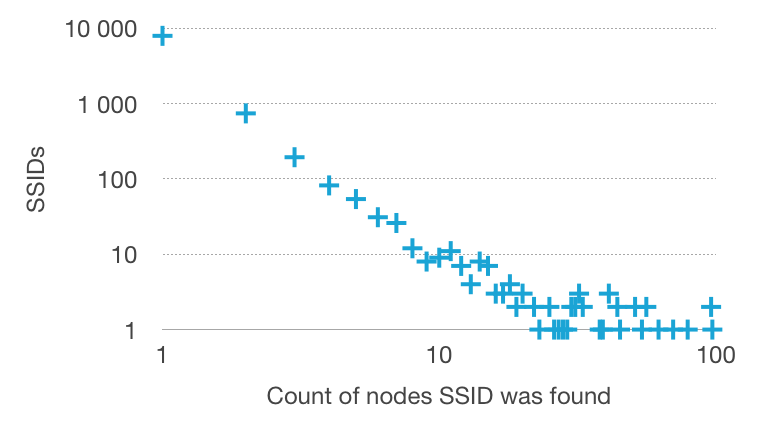
\includegraphics{images/nodes_per_ssid}
    \caption{From how many nodes a SSID was found. Note logarithmic scale.}
    \label{fig:nodes_per_ssid}
\end{figure}

In Figure~\ref{fig:ssids_per_node} we see how many SSIDs a node probed. Almost half of the nodes, 48~\%, probed only one SSID and are exluded from the graph. This behavior may be result of joining a network, and especially because mobile devices try to save battery, rejoining a network. Since we did not collect any other data than probe requests, this hypothesis is impossible to verify. After that, we see various number of probes between two and 15, but on sixteen nodes there is a very significant peak. As $16 = 2^4$, we believe that this is hard-coded limit on some devices. However, no single device manufacturer stand up: Apple, Samsung, LG and others are all presented in expected way in nodes with SSID count of sixteen.

\begin{figure}
    \center
    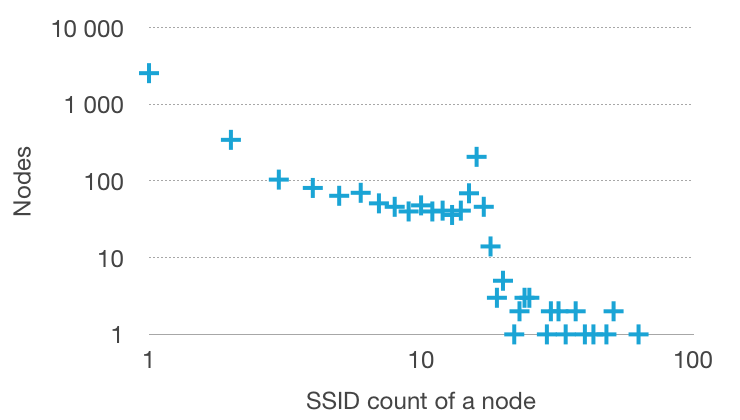
\includegraphics{images/ssids_per_node}
    \caption{How many nodes did a client probe. SSID count of one is excluded, having value of 1,174.  Also, 12 nodes had SSID count larger than 25, and are not visible in the graph.}
    \label{fig:ssids_per_node}
\end{figure}

We mapped devices also by manufacturer, since we can know it by the OUI part of the MAC address. We compared then our findings to the smart phone market share: this way, we could see if there were manufacturers with more insecure default settings than others. The market share was obtained from comScore's report for second quarter of 2014~\cite{comscore2014}

Manufacturer distribution is shown in Figure~\ref{fig:manufacturers}. Today's smartphone market in the U.S. is dominated by two largest players, Apple and Samsung. In our data, we see far more Apple devices than we should have expected: 57~\% of MAC addresses compared to 42~\% of market share. Also, Samsung is strongly underpresented in our data, with 10~\% of probes to 28~\% of market share. This suggests that owners of Apple iPhone leave their Wi-Fi on more often, or that Samsung uses passive scanning in many of its devices, or that Samsung users turn Wi-Fi off for some reason. This might be due to usage patterns, if iPhone encourages users to use wireless networks in some way. On the other hand, it is also possible that our target audience was biased towards Apple devices.

\begin{figure}
    \center
    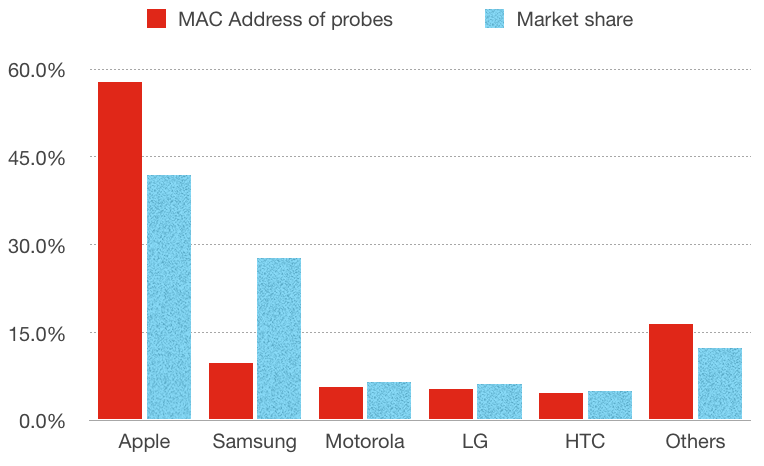
\includegraphics{images/manufacturers}
    \caption{Distribution of MAC addresses performing active scanning we found by manufacturer, and U.S. smartphone market share\cite{comscore2014}}
    \label{fig:manufacturers}
\end{figure}

For Twitter, we collected 10~\% of continuous feed from January 2014 to August 2014. After that, we filtered out all the results without geolocation data. In the end, we had 164 million tweets -- posts to Twitter -- in the database.

\section{Clustering}
\label{sec:practical_clustering}

We tried to find clusters from the data by using various methods. By finding clusters, we were looking if we could discover patterns. For example, do some SSIDs appear often together, and what it could tell us?

First, we calculated the similarity matrix of nodes by looping through all pairs. For similarity metric, we used Jaccard Index and Psim-3, as specified in Section~\ref{subsec:clustering}. After that, we run the actual clustering algorithm, and interpreted results by forming a visual representation or connecting cluster calculation with SSID lists. Visualization gives us an overview how the data looks like, whereas connecting with data shows the semantic meaning.

Hierarchical clustering does not work well for this type of data. Too many nodes had exactly zero similarity, which yields to maximum distance (in hierarchical clustering, we need to use distance instead of similarity).

Markov Clustering (MCL) works better with the data. We first created clusters of client devices with MCL, and then looked at shared SSIDs in each cluster. SSIDs were scored and sorted based on the frequency they appeared in a cluster, that is, the most important SSID is the one that most clients share withing the cluster. 

First there are seemingly obvious connections, such as people using differently named networks within the same university or another organization, such as \texttt{UCSB Secure} and \texttt{UCSB Wireless Web}. By these, we can verify that our algorithm works at least on some extent, and can continue for further results. We see that there are definetely links between companies: we identified at least a few different restaurants, ice cream bars, hair salons and retail stores. Once again, the problem is the long tail of SSIDs: most of the SSIDs appeared only in a small number of devices, and defining connections is not reliable.

To obtain a graphical representation of the data, we used Gephi and its \emph{Force Atlas} method~\cite{bastian2009gephi}. Showing all the edges was too heavy task, so we filtered the least important out. With Prism-3 similarity method and $\text{threshold} = 0.1$, we got the result shown in Figure~\ref{gephi_01}.

\begin{figure}
    \center
    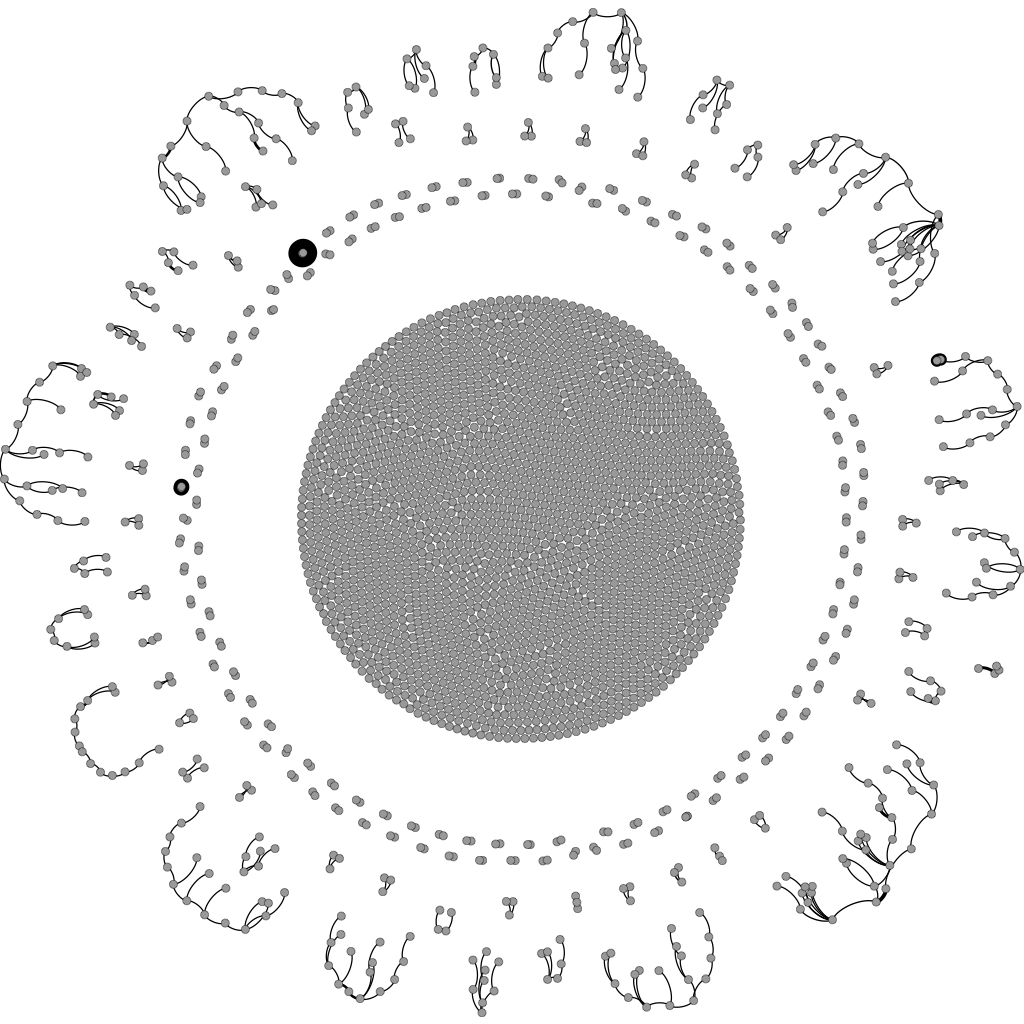
\includegraphics[width=\textwidth]{images/gephi-01.png}
    \caption{Graph created with Gephi. Nodes are client devices, edges are similarity between them calculated from SSIDs and using Psim-3 similarity metric with threshold $0.1$.}
    \label{gephi_01}
\end{figure}

The graph can be seen as having four rings. In the center there are lots of nodes with no important connections to anywhere: every node is its own cluster. Around those, there are lots of two-node pairs, followed by three-node clusters. Outermost we have clusters with many nodes. In the graph, darker edge represents higher similarity: there are a couple of extremely similar pairs.



\section{Combining data with third party services}
\label{sec:practical_thirdpartt}

For the rest parts of the experiments, we needed more details for our data. We developed an analysis framework, where our workflow was the following:

\begin{enumerate}
    \item Filter out devices with less than four probes; we do not believe to achieve anything by analyzing too small datasets.

    \item Get location data from WiGLE by SSID
    
    \item Calculate score for uncertainity of the location data:
        $$ u_{Loc} = C_1 \cdot \ln n + C_2 \cdot d^2 $$
        where $n$ is number of different locations for the SSID, $d$ is the average distance between locations, and $C_1$ and $C_2$ are constants. This way, there are small penalty for large number of networks with the same SSID, and larger penalty if they are far away from each others.
    
    \item By location data and SSID, query Google Places to find out if the location is a well-known place. SSID was splitted into different words by several delimiters, such as `-', `\_', whitespace, and case changes. For example, SSID \texttt{FourSeasons\_Guests} splits into three search terms, \texttt{Four}, \texttt{Seasons}, and \texttt{Guests}.

    \item Query Yelp database to get pricing information with same kind of parameters than Google Places.

    \item If the SSID or data from Google suggested it to be a hotel, query Expedia database to get more details.

    \item Last, manually assign uncertainty score for Google Places result and Expedia hotel result, if present. For example, if for SSID \texttt{BW PLUS VICTORIA PARK SUITES} our system gave a hotel called ``Best Western Plus Victoria Park Suites'' as a result, we can consider that really trustworthy.
\end{enumerate}

In Table~\ref{tab:stage_counts} there are counts of SSIDs processed in every phase. We see from the table, that even though we were able to get location infromation for three-quarters of SSIDs, less than half of the locations were considered accurate enough. This is due to ambiguous SSIDs: they appear more than once and in various locations.

\begin{table}[h]
    \center
    \begin{tabular}{|l|c|c|}
        \hline
        Unique SSIDs                            & 8454 & --- \\ \hline
        Unique SSIDs for devices with more than 3 probes                                  & 7271 & 100~\% \\ \hline
        Location point for SSID                 & 5451 & 75~\%  \\ \hline
        Reasonable low uncertainty for location & 2283 & 31~\%  \\ \hline
        Google Places data                      & 1543 & 21~\%  \\ \hline
        Trustworthy Google Places data          & 1016 & 14~\%  \\ \hline
        Pricing data (Yelp)                     & 633  & 8.7~\%  \\ \hline
        Detailed hotel information              & 389  & 5.3~\% \\ \hline
        Trustworthy hotel information           & 222  & 3.1~\% \\ \hline
    \end{tabular}
    \caption{SSID count for specific phses of analysis}
    \label{tab:stage_counts}
\end{table}

\subsection{Price ranges}
\label{subsec:practical_prices}

It would be very valuable to know if users are willing to pay more, or if they are looking for the cheapest alternative. We can try to fetch a rough approximation from SSID list: it is a reasonable hypothesis, that if the user has visited many expensive hotels and restaurants, she is ready to spend money on high-end products.

We fetched pricing information from Yelp~\cite{yelp}, which reports price range for places in four-step scale, from one to four. This is a helpful feature, because then we need not to normalize the prices between different cities or different types of services (such as hotels or restaurants).

To increase the accuracy of price range analysis, we discarded the results with high uncertainty for location or Google Places data. Also, most of the users had only one or two SSIDs with pricing information, and we discarded those too. As a result, we managed to calculate average price range for 328 users (11~\%).

The distribution of price average is shown in Figure~\ref{fig:prices_users}. We see a big peak on range $2.0 - 2.49$, and only five users had an average of at least 3.0. This may be a result of nature of Yelp data. Nonetheless, we believe that in many cases the result gives hints about customer's purchasing power or consuming behavior, accuracy correlating with the number of SSIDs where pricing data was found.

\begin{figure}
    \center
    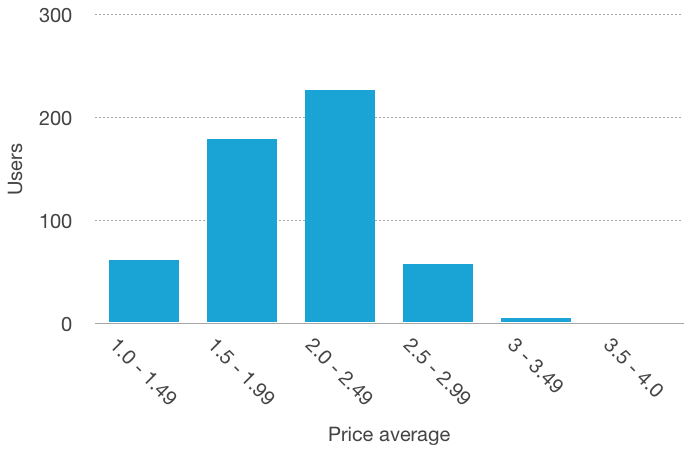
\includegraphics{images/prices_users}
    \caption{Distribution of price average}
    \label{fig:prices_users}
\end{figure}

\subsection{Discovering hometown}
\label{sec:practical_geolocation}

One task was to find out where a user comes from. Our hypothesis was that most of the people are from California, where the data was collected, but significant number of people probably are foreigners due to the tourist-friendly nature of area. Here, we define hometown as a place where user has spent most of his time lately: that is, if a German is visiting U.S., his hometown is still in Germany -- but if he has lived in California for a couple of years, his current hometown can be considered to be in California.

The problem is that SSID list does not give any information about number of times the network was used. We obtain absolutely same information if user has connected to the network once or a thousand times.

To get results, we used the following method:
\begin{enumerate}
    \item Filter out location results with too large uncertainty.
    \item Filter out hotels: we assume that people do not go to hotels in their hometown.
    \item Calculate the number of remaining locations, grouped by country and state.
    \item If large enough fraction of locations is from a specific place, consider that as user's hometown.
\end{enumerate}

We verified our results by manually going through SSID lists of users marked as foreigners. Generally, we have good reasons to believe that they were correct. In many cases, there were SSIDs that appear in WiGLE's database only once, or ones that are named after local business. For instance, one with SSIDs shown in Table~\ref{tab:example_hometown} was categorized as being from Stockholm, Sweden.

\begin{table}
\center
    \begin{tabular}{*{5}{l}}
    \\
SSID                 & City          & Country & State/County   & Uncertainty  \\ \hline
\hline
Danhostel.Copenhagen & Copenhagen    & DK      & Capital Region & 0.00 \\ 
\hline
ForumNacka           & Nacka         & SE      & Stockholm      & 0.00 \\ 
\hline
Sophiahemmet Guest   & \"{O}stermalm     & SE      & Stockholm      & 0.00 \\ 
\hline
TELE2INTERNET-2924   & Solna         & SE      & Stockholm      & 0.00 \\ 
\hline
Taby\_Centrum\_WIFI  & T\"{a}by          & SE      & Stockholm      & 0.00 \\ 
\hline
The\_Sandman\_Inn    & Santa Barbara & US      & California     & 0.00 \\ 
\hline
LAX-WiFi             & El Segundo    & US      & California     & 0.69 \\ 
\hline
free-hotspot.com     & Villeurbanne  & FR      & Rhone-Alpes    & 100.30 \\ 
\hline
DOVADO               & Uppsala       & SE      & Uppsala        & 128.03 \\ 
\hline
AWG-WiFi             & Warwick       & US      & Rhode Island   & 2763.57 \\ 
\hline
home47               & Solntsevo     & RU      & Moscow         & 5412.23 \\ 
\hline
NETGEAR81            & Escondido     & US      & California     & 6144.63 \\ 
\hline
    \end{tabular}
    \caption{User with this SSID list was categorized to be from Stockholm, Sweden. Last five locations were not included in calculation due to high uncertainty.}
    \label{tab:example_hometown}
\end{table}    

We run the analysis for nodes that had probed at least four different SSIDs, which is 870 nodes. Hometown was succesfully calculated for 618 (71~\%) of them. For 347 nodes (56~\% of succesfuls) it resulted as California, and 81 (13~\%) were identified as foreingers. If hotel results are included in results, number of identifications increases, but all the new results are categorized as Californians. Therefore, we can say that most of them are likely visiting the area, and must be excluded from the results.

\subsection{Social media networks}
\label{sec:practical_social}

We tried to identify users from social media networks based on their SSID history and location data included in social media postings. We found that in general case this is not possible.

To see why this is the case, consider first our data. We have three datasets: user's SSID history, SSID-location mapping, and social media database. For every dataset, let's consider possible errors they have and coverage of population.

The first is considered error-free: we have succesfully captured possible SSID probes, and filtered erroneous out with the checksum field (FCS) of 802.11 standard. Coverage could be increased with time, better antennas, and better capture positions, such as larger cities.

The second dataset, SSID-location mapping, is more problematic. As shown in Table~\ref{tab:stage_counts}, we got location data for about 64~\% of SSIDs. However, the accuracy and reliability of SSIDs shrink fast, and only 27~\% of them can be thought as reasonably trustworthy. Even in that part of data, there are small errors, for example GPS errors in the city or due to fact that location of measuring device is not the same as location of access point.

The third dataset, social media database, can be considered pretty accurate. The location features of a smartphone are reasonably good, even though small errors from GPS can occur, as in previous case. The bigger problem is the coverage of data: we were able to obtain only 10~\% of total Twitter feed in 2014. Furhter, only about 1~\% of tweets included location data, as including location to tweets is a setting controlled by user, and off by default. Thus, we had only 0.1~\% of total tweets to analyze and try to find the user. Also, Twitter is a relatively small media: in 2013, 18~\% of online adults used it, whereas Facebook scored as high as 71~\%~\cite{pew_socialmedia}, and some of those users are only occasionally following it without posting anything.

In dense areas such as in the center of a city, there are multiple wireless networks overlapping. Thus, a tweet from a specific location cannot be bound to a single wireless network, which yields higher amount of false positives.

The identification might work, if special circumstances were met. The most important of these is to post to social media from a location where only small number of people has tweeted (sparsely populated area) --- but not too sparsely, so that the SSID database has its location. Also, a unique travel path would reveal the identity: a tweet from middle-sized city from Finland is not enough to identify an individual, but if the same person has tweeted also from mid-size town from U.S. west coast and northen Italy, odds are high that there are not many people having done so.

\section{Other findings}
\label{sec:practical_other}

As noted while studying legal issues on Chapter~\ref{chapter:legal}, someone might name his network after his own name. We looked the data we had captured to find such networks. In fact, we found 24 SSIDs that were form of \texttt{[firstname] [lastname]'s [network|own network|etc]}, of which 22 were named after different individuals, one was duplicate, and one was after a family name.

To further study these cases, we tried to identify these people by searching their name from various public sources and social media. As the names of people are not unique, we assumed that they were living in a reasonable distance from capture area. We believe that we found the correct individuals in 13 cases; in three cases we found too many results to uniquely identify a person; and six SSIDs did not result to a match.

We found also 33 WPS leaks, specified in Section~\ref{sec:wps}. Sadly, the phone names in the leaks looked like default names, which the owner had not changed. Most of the leaks were from Motorola devices, bought from Verizon.


\section{Conclusion of practical study}
\label{sec:practical_conclusion}

This chapter provided valuable information of how feasbile it is to perform profiling techniques based on SSID list.

The first observation was that majority of clients seen were not performing active scanning. Also, this varied between manufacturers: in our data, Apple devices were overpresented compared to their market share, whereas Samsung had relatively low presense in the data.

We saw that it is very difficult to identify users from social media based on SSID list. Such an action requires lots of resources, most likely direct access to social media database in question. Also, currently only a small minority of users are including their location in their postings -- in Twitter, it seems to be about on percent. Thus, odds to find an individual are very low.

However, we showed that it is possible to form behavioral patterns based on SSID list. We succesfully ran graph clustering algorithm, that showed plausible links between networks and companies. We were successful to discover user's possible hometown. By using third-party services, we also created our hypotheses on users' willingess to pay for high-end services.

In a conclusion, we showed that profiling is possible, but only for relatively small portion of population.

%%%%%%%%%%%%%%%%%%%%%%%%%%%%%%%%%%%%%%%%%%%%%%%%%%%%%%%%%%%%%%%%%%%%%%%%%%%%%%%


\chapter{Countermeasures}
\label{chapter:countermeasures}

Not everyone is happy or comfortable with an idea that someone is tracking their movements or profiling their behavior. Together with a legal view presented in Chapter~\ref{chapter:legal}, we will study technical countermeasures to prevent the usage of techniques discussed in this paper. 

\section{Countermeasures for MAC address tracking}

Tracking customers' movements based on MAC address is a relatively simply technique, as we have already seen. Tracker needs to be able to (1) locate a device, and (2) combine togheter individual location points from the same device.

We cannot prevent anyone from locating a device that transmits signal on radio frequencies, so the only possible countermeasure is to negate possibility to match location points to a single device. Therefore a device must not broadcast MAC address or other information that uniquely identifies it.

Current WLAN standard offer no help as they mandate sending a MAC address with every request, so there is a need for new solutions. Apple announced in June 2014 that in iOS 8, it will randomize the MAC address during wireless network scanning~\cite{FredericJacobs2014,apple_wwdc_privacy}. A randomized address would work as a \emph{pseudonym}, which identifies device for a specific request or for a limited time, but not universally.

As iOS 8 is not yet released, we cannot study its behavior in detail. However, randomization presents a couple of interesting questions. Normally, a device sends a bunch of probe requests almost at once and then sleeps for some period of time, usually between 30 to 60 seconds. A proper implementation requires that the MAC address is randomized after \emph{every} single probe request, not only between different cycles. Otherwise, tracker could identify device based on the broadcasted SSID list and completely ignore the MAC address.

To be a working solution, it must not use too much resources. A device with randomized MAC address needs to save all the previous addresses in order to be able to filter replies targeted to it. Because number of different networks is really small, this will not be a pjroblem. Also, after a succesful connection or relatively short timeout (measured in seconds), a pseudonym can be forgotten. Some computational overhead will be generated from randomizing process, but that should be really small -- after all, we are only generating 24 or 48 bits, depending on whether we randomize also OUI part or not.

We should look if there is enough space for randomizing a new MAC address for every probe request without collisions. Suppose that an average device has $N = 8$ SSIDs on their preferred network list, which is a safe assumption based on our dataset. By randomizing only organizationally-controlled part of MAC address -- leaving OUI untouched, respecting its purpose -- a single OUI block can provide about 16 million different addresses, and give enough space for
$$M = \frac{2^{24}}{8} \approx 2*10^6$$
simultaneous devices. Due to birthday paradox, this number needs to be decreased. The number of devices to success without collision for probability $p$ can be approximated by formula~\cite{mathis1991generalized} 
$$n \approx \sqrt{\frac{1}{4} - 2 \cdot M \cdot \ln p}$$ 
which gives us the results presented in Table~\ref{tab:prob_random}. As we see, the number of devices decreases rapidly when we raise probability requirements: for 99.9~\% probability for no collisions, only 65 simultaneous devices are allowed.

However, we should remember that not all devices are in the same OUI block. Apple, who has more than 40~\% of market share in the U.S.~\cite{comscore2014}, has more than 300 OUI blocks reserved. Because the number of devices is proportional to square root of the size of address space, 300 times more addresses would give about 17 times more devices with same collision probability. Therefore, the numbers in the table can be multiplied by 20 (there are also other vendors than Apple), and we should be safe even for larger networks.


\begin{table}[ht]
\center
\begin{tabular}{|l|r|}
    \hline
    $p$ & $n$   \\ \hline \hline
    0.5 & 1705  \\ \hline
    0.9 & 665   \\ \hline
    0.95 & 464  \\ \hline
    0.99 & 205  \\ \hline
    0.999 & 65  \\ \hline
    0.9999 & 20 \\ \hline
\end{tabular}
\caption{Number of devices $n$ with the same OUI to survive simultaneously in a same network, without collisions, with probability $p$, when randomizing only 24 bits of the MAC address.}
\label{tab:prob_random}
\end{table}

Randomization can be more stealthy if the whole address is being randomized, including the OUI part. This way, tracker could not determine straight from MAC address which device it is. Spoofing such a field can be a double-edged sword: some services might rely on manufacturer identification and stop working after such a spoof. However, this is pretty unlikely. Randomization should happen only in scanning phase, and after joining a network, it will not change anymore.

A direct consequence of previous is that after joining a network, a device can be tracked again, since it sends packets with a non-volatile MAC address. The MAC is not secured against eavesdropping in encrypted wireless networks. The question that remains open is whether the device uses a fixed MAC for every session or continues with the last randomized one. Obviously, a randomized address for every session would be better for privacy.

A possible problem may be that the device is leaking other information where it can be identified. For example, the WPS protocol presented in Section~\ref{sec:wps} might leak new unique user identifier, which renders the whole defense meaningless.

Implementing MAC address randomization seems to be a promising countermeasure against tracking during the scanning phase, if implemented correctly. Joining a network removes the advantage of randomization.

\section{Countermeasures for SSID profiling}
\label{sec:countermeasures_ssid}

SSID profiling depends on a few factors. A profiler has to be able to \begin{enumerate}
    \item Record SSID probes,
    \item Identify which probes are sent from the same device, and
    \item Analyze them using various data sources.
\end{enumerate}

If we want to prevent an attacker from recording SSID probes, we must not send them at all. This can be done using passive scanning, specified in Section~\ref{subsec:passive_scanning}, or with active scanning with a wildcard SSID, discussed in Section~\ref{subsec:active_wildcard}.

Passive scanning may have performance problems, since a node needs to wait for APs to advertise themselves, instead of probing them. As manufacturers would like to give customers best possible user experience, and significant delays joining a network could result in worse experience, this may not be a feasible solution. Manufacturers could make this as a setting in the device to give users a fast experience initially, with option for privacy-concerned users to turn their device into passive scanning or wildcard mode.

With active scanning using wildcard SSID, an attacker cannot anymore eavesdrop SSIDs exchanged. However, it might be possible for a determined one to probe the client with many different alternative SSIDs and see which ones a node is willing to join. The scale of data transmission required will render this attack useless for profiling cases, but man-in-the-middle attack presented in Section~\ref{sec:mitm_probes} could probe a node with most common SSIDs --- it needs to match only one of them to perform attack.

Third way to limit exposure is to probe only networks that are physically near the node. This approach is briefly introduced in work by Kim et al.~\cite{kimposter}, where a node knows its own location and the location of APs it has connected previously. Therefore, the node can try to actively probe only APs that should be available, and passively listen for others' probes. 

This approach suffers from a couple of issues. First, it requires node to know its own location, which may take some time to resolve resulting worse user experience. Second, the requirement for location data forces user to keep his GPS on, which consumes battery -- an important constraint on mobile devices. Third, storing previous AP's location data on mobile device might cause new privacy issues for stolen device: an SSID-to-geolocation mapping is not anymore required, but a thief can easily see where user has visited. Fourth, if GPS is not available, which is the case indoors, they propose that node could determine its location by neighboring APs' signatures. This is not a very reliable way, and may lead to worse user experience, which prevents any manufacturer to implement the feature.

We can allow devices to transmit data but render it useless for eavesdroppers using cryptographic techniques. Research by Lindqvist et al.~\cite{lindqvist2009privacy} proposes a method for that by modifying protocol to join a wireless network. In their work, a client includes its nonce $N_{client}$ in a probe request. Then AP sends back client's nonce, its own nonce $N_{AP}$, and a random identifier that acts as an SSID for the connection, called R-SSID. The R-SSID is encrypted using shared key, and the key is generated from shared secret, network passphrase.

There are ways to render previous defenses ineffective. Achara et al. noticed that the SSID list can be fetched by smartphone app with specific permissions.~\cite{2014_WISEC_Achara} There, the app access directly the SSID list in the phone's storage, and is able to fetch it remotely. Users can choose not to grant such permissions, but we have serious doubts on leaving security to rely on a single ``OK'' click.

To negate the second requirement, identifying which probes are sent from the same device, we can use the same technique as in previous section, MAC address randomization. If the MAC address is randomized for every probe, the only thing a profiler sees is single requests from different MAC addresses. It would need to identify devices in some other way, so we need to be sure that no additional information is leaked --- just as discussed in previous section.

The third option, preventing analyzing, cannot be done in technical measures. 


\section{Securing against active attacks}

In the following, we will look at how to secure against active man-in-the-middle attacks presented in Chapter~\ref{chapter:attacks}. 

Defense mechanisms can be categorized into two groups. In client-side defenses, mobile nodes take new security precautions to avoid connecting to rogue access point. In network administrator's defenses, the administrator of WLAN is trying to actively locate rogue access points in his own network. After detecting one, other technical and non-techincal actions can be taken in order to remove the access point.

\subsection{Client-side defenses}

Man-in-the-middle attacks presented here require that user connects to a rogue access point. In the first case, an access point was open, which means that some operating systems will connect to it without user's consent. Obviously, this threat can be negated by turning such a feature off. 

In evil twin attack, the attacker has learnt a SSID of an existing access point and presents himself as with the same SSID. For this, a node could save each SSID with a BSSID, AP's MAC address. Therefore the node would detect that there is a different physical device with a different MAC address, and present two alternative ways to proceed:
\begin{enumerate}
    \item Try to search harder, wait a moment: maybe there is a legitimate AP available. If so, connect to it.
    \item If not, it is possible that network equipment has been upgraded, or the network spans over a larger physical area with lots of access points. In that case, a mobile device could present confirmation dialog to the user, asking if he really wants to connect to that network. This approach is present at least on Windows Phone 8.
\end{enumerate}

Song et al.~\cite{song2010peeping} suggest that client could look for network hops. Their defense addresses the situation where there is an evil twin between the legitimate AP and the client. In other words, th evil twin is using the original WLAN for internet connectivity. When this is the case, the client could detect that in a network with two different APs with the same SSID, one has one hop more to the internet than another. Therefore, it can know that an extra hop is for MITM attack, and should not connect there.

Song's approach works well when their assumptions hold. It is reasonable to think that their use case is a realistic one, but one should not base full trust on it. First, with today's cellular connectivity (3G, 4G), the evil twin may easily be connected to internet without utilising the original AP's internet connection. Second, the evil twin may be located somwhere else: for example, someone could setup a ``Starbucks WiFi'' where there is no Starbucks nearby, but quite a many may join the network since they have previously visited Starbucks.

To tackle the previous Starbucks scenario, Gonzales et al.~\cite{gonzales2010practical} propose two methods. First, they want to combine trust with location data: if the network is seen on a different place than initially, it may be evil. The location is determined by looking for other APs nearby: if too many of them have changed, the location is tought to be different. The second method requires protocol changes, as they propose that APs should be identified with public key cryptography. Keys would be self-signed without trusted third party, which means that initially there is \emph{no verified trust}, but all the later connections are guaranteed to be with the same AP as the first one. The approach is called \emph{trust-on-first-use}, and is used also in SSH protocol. Similiar kind of method is proposed by Bauer, Gonzales and McCoy~\cite{bauer2008mitigating}.

Often best solutions are simple. Consider the scenario when attacker is exploiting user's probe requests to guess a name of network user would be willing to connect to. Then the defense is straightforward: do not send probe requests with SSIDs, but resort to wildcard probing or passive scanning. A problem with passive scanning is that it may reduce performance, which manufacturers do not like to see. However, active scanning with wildcard SSID should be fast enough.

An attack for previous defense would be to guess a few most used SSIDs and try to connect with them. Here saving a BSSID with an SSID would help: guessing a SSID from, say, out of twenty most common used ones is trivial, but going through the MAC address is not. Even if attacker would be limited to a couple of OUIs by guessing correclty the manufacturer, it has still 24-bit keyspace to discover, which is more than 16 million possibilities.

In a conclusion, there are lots of different approaches for defending user against evil twin attacks on the client side. None of them is perfect: some require changes to protocol which may be troublesome to deploy; some work only on some scenarios, and attackers knowning that limitation can easily change their way to attack. The best defense is achieved by combining many different approaches, and can be thought as \emph{defense in depth} with many layers.

\subsection{Network administrator's defenses}

In addition to user's efforts, network administrators can try to detect rogue APs around their network. This field is much more mature in terms of commercial solutions than client's side, which may be due to the fact that it is easier to sell security solutions to techinical administrators than to poorly-educated consumers. Manufacturers include most of big vendors in wireless and networking industry, such as Motorola~\cite{motorola_airdefense} and Cisco~\cite{cisco_ips}. Unfortunately companies do not usually disclose the details of their implementations.

The first type of administrator-side defenses monitors waves on radio frequencies (RF) to find rogue APs. The idea behind this method is simple: there are only a known amount of wireless access points in known locations with known BSSIDs, and everything else is unauthorized. The method is therefore comparing scanning results to a whitelist. The scanning can be done my walking around with a laptop or installing probing devices around the building.~\cite{proxim_rogue_ap}

There are also solutions that combine access points with a probing device. Together with that, they may monitor the wired network and try to correlate the signals.~\cite{proxim_rogue_ap} If some data is seen only on wireless network but not on wired, it is clear that this AP is not set up by the administrator. If it tries to look legitimate, for example by having the same SSID, one can make a guess that it is a rogue AP.

Another possibility to detect rogue APs would be to measure round-trip time (RTT) to a known router inside the network as shown in work by Watkings et al.~\cite{watkins2007passive} The approach exploits the fact that time difference can be measured when packet travels through an extra hop. Thus, the last approach is actually the same as presented in previous section for user-side defenses to detect an extra hop, just with administrator's devices.

Both of these methods require network administrator to deploy his monitoring devices around the area network covers which can be expensive. To solve this particular problem, Bahl et al. from Microsoft propose~\cite{bahl2005dair} that in an office environment, existing desktop computers could have cheap wireless USB devices and use their spare CPU time to detect unknown APs. As desktop workstations are normally connected via wired network, the wireless connectivity would be available for only monitoring purposes.

\subsection{Conclusion of active attacks defenses}

In a conclusion, we can say that there are numerous types of users and threats. The ones a regular traveler may face are somewhat different from the ones a network administrator in a big company encounters, even though the basic idea and technology is pretty much the same.

No single silver bullet exist to mitigate all the threats. The best result is achieved with defense in depth by having multiple layers of defenses that complement each others.

Having said that, we must note that leaving active probing on increases attack surface significantly. The easiest defense is to use wildcard probing or passive scanning.


%%%%%%%%%%%%%%%%%%%%%%%%%%%%%%%%%%%%%%%%%%%%%%%%%%%%%%%%%%%%%%%%%%%%%%%%%%%%%%%


\chapter{Conclusion}
\label{chapter:conclusion}

In the beginning of the thesis, in Chapter~\ref{chapter:protocol}, we described terminology and concepts of wireless networks. We identified a couple of important identifiers, the MAC address and the SSID. We also studied packet formats in detail, and saw how wireless devices find the network they want, and how they join it. We had three possibilities: passive scanning, active scanning, and active scanning with wildcard. Active scanning is the same as active probing.

In Chapter~\ref{chapter:profiling}, we discussed how and why someone could track and profile users based on probes emitted from their wireless devices. We discussed on concepts of locating a device, either a node inside a wireless network, or an access point globally using huge databases. We also saw different methods on profiling users, such as discovering real-life relationships, clustering data with well-known graph algorithms, and comparing data with third-party services. We also looked how a WPS protocol can leak some information.

After passive profiling, in Chapter~\ref{chapter:attacks} we discussed ways to perform active man-in-the-middle attacks. All the attacks share the same basic idea, attacker being between user and a legitimate service. We saw numerous way to do so, and discovered that there are easy-to-use, off-shelf devices available even for attackers with low skills. Thus, we consider these attacks to be extremely feasible to perform, and they must be taken seriously.

Having studied techinical views, we looked on legal status of the discussed techniques on Chapter~\ref{chapter:legal}. Especially we focused on Google's Street View case, which is the best-known example of these issues, even though it does not address them in every way we would like to -- metadata collection has not been discussed on that case. We found that European Union legislation is much stricter than one in the United States, and that officials in the EU -- the Article 29 Working Group -- has taken really strong position on suggesting that all wireless network data should be treated as personal data, which makes huge burdens on companies to collect and use it. On the other hand, legislation is really permissive in the U.S. as long as it handles only metadata without actual messages, and allows even more if the analysis is not made public. However, we see that there might be oncoming changes on U.S. laws which would bring them closer to European counterparts, but the process is far from complete.

In Chapter~\ref{chapter:practical} we conducted a practical experiment on techniques studied in Chapter~\ref{chapter:profiling}. We saw that majority of devices, 77~\%, had only wildcard scanning enabled, and can not be profiled. However, this does not prevent tracking, as the device is leaking its MAC address all the time. Naturally, we cannot know how many had only passive scanning enabled or turned their WLAN connectivity off, since those devices do not emit anything we could have captured.

We saw that it is possible to find out some charasteristics of users based on their SSID list. Examples included discovering their hometown and if they favored high- or low-end restaurants and hotels. Still, the biggest problem with these findings is that they apply only to small percentage of the population: only small number of people have mobile device with active scanning, only some number of SSIDs can reliably resolve to a location user has visited, and for only some number of those we find pricing or other relevant information. Thus, large-scale profiling and gaining benefits in practise is not straightforward.

We also discovered that it is really difficult to find users from social media based on their SSID list. The biggest problem is that there is no large enough public mapping from visit history to identity: however, there probably are closed ones in big companies, where we do not have access. Even after that, number of false positives would be high, as networks overlap a lot in densely populated areas, such as cities. We think that identification requires measures that are not likely reasonable to be used, which means that SSID list should not be considered personal data in terms of EU legislation. However, MAC address should be, as it may allow identification easily with accurate indoor-WLAN position systems and CCTV cameras, and it is much more stable than SSID list.

In the end, in Chapter~\ref{chapter:countermeasures}, we found that there are many countermeasures available. As short-term solutions, manufacturers should stop using active scanning but turn to wildcard or passive ones. At least there should be a private mode available, so that users could choose if they wanted to expose previous SSIDs to everyone or not. In medium term, MAC address randomization could be a working solution, and Apple is very soon launhing a new mobile operaing system with it. In long term, protocol changes would be required, and there have been propsals on them.

% Load the bibliographic references
% ------------------------------------------------------------------
% You can use several .bib files:
% \bibliography{thesis_sources,ietf_sources}
\bibliography{sources}


% Appendices go here
% ------------------------------------------------------------------
% If you do not have appendices, comment out the following lines
% \appendix


% End of document!
% ------------------------------------------------------------------
% The LastPage package automatically places a label on the last page.
% That works better than placing a label here manually, because the
% label might not go to the actual last page, if LaTeX needs to place
% floats (that is, figures, tables, and such) to the end of the 
% document.
\end{document}
